\documentclass[english, 12pt, a4paper, elec, utf8, a-2b, online]{aaltothesis}

%% DO NOT MOVE OR REMOVE \setupthesisfonts
\setupthesisfonts

%%
%% Add here the packges you need
%%
\usepackage{graphicx}
\usepackage{algorithm}
\usepackage{algpseudocode}
\usepackage{amsmath}
\usepackage{amsfonts}
\usepackage{subcaption}
\usepackage{cleveref}
\usepackage[most]{tcolorbox} % loads tcolorbox with many default libraries
\graphicspath{{/media/tianxing/Shared Volume/studies/aalto_MSc/HPC_thesis/mpc_in_practice/impl/figs/}}
 

%% For tables that span multiple pages; used to split a paraphrasing example in
%% the appendix. If you don't need it, remove it.
\usepackage{longtable}

%% A package for generating Creative Commons copyright terms. If you don't use
%% the CC copyright terms, remove it, since otherwise undesired information may
%% be added to this document's metadata.
\usepackage[type={CC}, modifier={by-nc-sa}, version={4.0}]{doclicense}
%% Find below three examples for typesetting the CC license notice.


%% Edit to conform to your degree programme
%% Capitalise the words in the name of the degree programme: it's a name
\degreeprogram{Computer, Communication and Information Sciences}
%%

%% Your major
%%
\major{Algorithms}
%%

%% Choose one of the three below
%%
%\univdegree{BSc}
\univdegree{MSc}
%\univdegree{Lic}
%%

%% Your name (self explanatory...)
%%
\thesisauthor{Tianxing Wu}
%%

%% Your thesis title and possible subtitle comes here and possibly, again,
%% together with the Finnish or Swedish abstract. Do not hyphenate the title
%% (and subtitle), and avoid writing too long a title. Should LaTeX typeset a
%% long title (and/or subtitle) unsatisfactorily, you might have to force a
%% linebreak using the \\ control characters. In this case...
%% * Remember, the title should not be hyphenated!
%% * A possible 'and' in the title should not be the last word in the line; it
%%   begins the next line.
%% * Specify the title (and/or subtitle) again without the linebreak characters
%%   in the optional argument in box brackets. This is done because the title
%%   is part of the metadata in the pdf/a file, and the metadata cannot contain
%%   linebreaks.
%%
\thesistitle{MPC in practice}
\thesissubtitle{MPC in practice}
\place{Espoo}
\date{10 July 2024}

\supervisor{Prof.\ Jukka Suomela}
%%

%% Advisor(s)---two at the most---of the thesis. Check with your supervisor how
%% many official advisors you can have.
%%
\advisor{Hossein Vahidi}
%%

%% Aaltologo: syntax:
%% \uselogo{?|!|''}
%% The logo language is set to be the same as the thesis language.
%%
%\uselogo{?}
%\uselogo{!}
\uselogo{''}

\copyrighttext{\noexpand\textcopyright\ \number\year. This work is 
	licensed under a Creative Commons "Attribution-NonCommercial-ShareAlike 4.0 
	International" (BY-NC-SA 4.0) license.}{\noindent\textcopyright\ \number
	\year \ \doclicenseThis}
%%%%%%%%%%%%%%%%%%%%%%%%%%%%%%%%%%%%%%%%%%%%%%%%%%%%%%%%%%%%%%%%%%%%%%%%%%%%%%%%
\newcommand{\mstalgo}{$MST\_\log\log{n}$}

\keywords{Distributed computing, Supercomputing, Congested clique, MST, Puhti, MPI, CUDA, MPC}

\thesisabstract{
This thesis investigates the performance of Congested Clique algorithms on modern supercomputers, specifically Puhti, a Finnish supercomputer hosted by CSC.\\
The study focuses on a representative algorithm, \mstalgo{}, which is implemented using two different programming paradigms: OpenMPI (Message Passing Interface) for CPUs and CUDA (Compute Unified Device Architecture) for GPUs. The goal is to evaluate the compatibility of modern computing architectures with the Congested Clique model.\\
The evaluation examines several aspects, including how distributed computation and communication in the Congested Clique model are translated to supercomputer architectures, the overhead introduced by this translation, and the extent to which the theoretical time complexity of the algorithm holds in practice.\\
MPI is a standardized and portable message-passing library interface widely used for parallel computing, while CUDA is a parallel computing platform and programming model developed by NVIDIA for general-purpose computing on GPUs.\\
}
% result: TODO


%% All that is printed on paper starts here
%%
\begin{document}

%% Create the coverpage
%%
\makecoverpage

\makecopyrightpage

\clearpage

\begin{abstractpage}[english]
	\abstracttext{}
\end{abstractpage}

\newpage

\dothesispagenumbering{}

\mysection{Preface}
I want to thank Professor Jukka Suomela and my advisor Hossein Vahidi for their guidance.

I also want to thank my friends for keeping me sane and alive.

\vspace{5cm}
Otaniemi, 10 July 2024\\

\vspace{5mm}
{\hfill Tianxing Wu \hspace{1cm}}

%% Force a new page after the preface
%%
\newpage


%% Table of contents. 
%%
\thesistableofcontents


%% Symbols and abbreviations
\mysection{Symbols and abbreviations}


\subsection*{Abbreviations}

\begin{tabular}{ll}
\mstalgo{}         & The algorithm described in \cite{MSTLogLogn} \\
MPI                & Message Passing Interface \\
CUDA               & Compute Unified Device Architecture \\
HPC                & High-performance computing \\
AI                 & Artificial intelligence \\
GPU                & Graphics processing unit \\
CPU                & Central processing unit \\
MST                & Minimum spanning tree \\
SLURM              & Simple Linux Utility for Resource Management \\
SM 							   & Streaming multiprocessor \\
SP 							   & Streaming processor \\
\end{tabular}

\cleardoublepage

\section{Introduction}
\label{sec:Introduction}

\thispagestyle{empty}
The Congested Clique model, as described in \cite{powerCongestClique}, is a framework for distributed computing. It consists of $n$ computing nodes arranged in a clique network, where each node is directly connected to all other nodes. In this model, each node in the network corresponds to a node in an input graph $G$, and the nodes collaborate to solve a problem on $G$.

The efficiency of the Congested Clique model is measured by the number of communication rounds required for an algorithm to converge. In each round, nodes perform local computations and exchange $O(\log{n})$ bits with their neighbors. The model emphasizes communication over local computation, as communication is considered the primary bottleneck in distributed computing. Local computation is assumed to be free, with each node having unlimited computational power and memory.

This study explores the Congested Clique model in the context of modern distributed computing hardware, specifically supercomputers. Supercomputers are high-performance machines designed to solve large-scale scientific and engineering problems. Unlike traditional computers, supercomputers utilize multiple processing units \cite{IBMsupercomputing}. Their distributed nature makes them well-suited for executing Congested Clique algorithms.

To evaluate the compatibility of modern computing architectures with the Congested Clique model, we implement a representative algorithm, \mstalgo{}, on a supercomputer. The implementation is carried out using two different programming paradigms: OpenMPI (Message Passing Interface) for CPUs and CUDA (Compute Unified Device Architecture) for GPUs.

\subsection{Methodology}
The algorithm \mstalgo{} from \cite{MSTLogLogn} is selected as the representative algorithm for this study. Its representativeness is discussed in detail in \cref{sec:mst_algo}. \mstalgo{} solves the Minimum Spanning Tree (MST) problem in $O(\log{\log{n}})$ communication rounds in the Congested Clique model. The MST problem involves finding a spanning tree of a graph $G$ with the smallest possible total weight. We demonstrate that \mstalgo{} is representative of algorithms designed for the Congested Clique model, and its properties generalize to the entire category of such algorithms.

To evaluate its performance, \mstalgo{} is implemented on Puhti, a Finnish supercomputer hosted by CSC \cite{Puhti}. The implementation is carried out using two distinct programming paradigms:
\begin{itemize}
	\item[--] Message Passing Interface (MPI) for CPUs.
	\item[--] Compute Unified Device Architecture (CUDA) for NVIDIA GPUs.
\end{itemize}

The choice of both CPUs and GPUs reflects the diversity of modern computing hardware. These platforms follow different programming paradigms and have distinct hardware constraints. While implementing \mstalgo{}, we adhere to best practices and optimize the implementation without altering the algorithm itself.

In the Congested Clique model, we assume that the graph to be solved is the same as the network graph, which is a complete graph. When implementing \mstalgo{}, we separate the network graph and the problem graph $G$ into two distinct graphs. Each node in the model is represented as a computing unit in our implementation, which can either be a physical CPU core/thread or a virtual computing resource assigned to the node. Nodes are not necessarily separate machines connected by a network; they can reside on a single computing core or thread. However, we ensure that each node can communicate with any other node in the network.

We do not allocate physically separate machines to the nodes in this work for two reasons: (1) it would be a waste of resources for a single node, and (2) the supercomputer does not have enough GPU/CPU nodes to allocate one per graph node. As we are dealing with large graphs, the graphs used in this study are complete graphs with $n$ vertices, containing $\frac{n(n-1)}{2}$ edges. The focus is on large graphs, with $n$ scaling up to $10^5$ and the number of edges reaching up to $10^{11}$.

\subsection{Objective}
The purpose of this work is to explore the connections between the Congested Clique model and modern distributed computing hardware, software, and tools. We present our approach to simulating Congested Clique algorithms on HPC hardware by making informed design decisions regarding the following aspects:
\begin{itemize}
	\item[--] How communication is handled across different programming paradigms.
	\item[--] How workload is allocated to nodes to maximize hardware utilization.
	\item[--] How communication is synchronized in a round-based manner.
\end{itemize}

The implementation of \mstalgo{} is detailed in \cref{sec:mpi} for MPI and \cref{sec:cuda} for CUDA.

We evaluate the performance of the simulation and analyze how hardware limitations affect the algorithm's performance in terms of memory, computation, and network constraints in \cref{sec:mpi_performance} and \cref{sec:cuda_performance}. Specifically, we address the following questions:
\begin{itemize}
	\item[--] What assumptions of the Congested Clique model lead to performance bottlenecks.
	\item[--] Under what settings do these bottlenecks appear.
	\item[--] Under what conditions does the algorithm perform as expected by the Congested Clique model.
\end{itemize}

We compare the performance of \mstalgo{} with its sequential alternative in terms of:
\begin{itemize}
	\item[--] Capability to process large graphs with a high number of vertices and edges.
	\item[--] Wall clock time when processing the same graphs.
\end{itemize}

Finally, we discuss the scalability of \mstalgo{}:
\begin{itemize}
	\item[--] Strong and weak scaling: How adding more nodes speeds up computation and which hardware components become bottlenecks as scaling continues.
	\item[--] Time composition during scaling: How the runtime is distributed between MPI communication and local computation. Does the time complexity align with theoretical expectations?
\end{itemize}
\clearpage

\section{Preliminaries}
\label{sec:preliminaries}

\subsection{Congested clique (also known as CLIQUE)}
The Congested Clique model is a theoretical framework for distributed computing, where \( n \) nodes are fully connected, forming a complete graph. Each node is assigned a unique identifier that requires \( O(\log{n}) \) bits for representation. The network operates in synchronized communication rounds, where all nodes begin and complete each round simultaneously. During a single round, each node performs local computations and communicates with its neighbors by sending at most \( O(\log{n}) \) bits to each of them. Communication is achieved through unicast, allowing a node to send distinct messages to different neighbors over its links within the same round. This model emphasizes communication efficiency, as the nodes are assumed to have unlimited computational power and memory resources. Consequently, the primary metric for evaluating algorithm performance in the Congested Clique model is the number of communication rounds required, rather than the time spent on local computation. \cite{powerCongestClique}
\subsection{\mstalgo{}}
\label{sec:mst_algo}
\mstalgo{} is an algorithm developed by Zvi Lotker, Boaz Patt-Shamir, Elan Pavlov, and David Peleg in 2005 \cite{MSTLogLogn}. It solves the Minimum Spanning Tree (MST) problem in $O(\log{\log{n}})$ communication rounds within the Congested Clique model.

The algorithm begins by partitioning the nodes of the graph \( G \) into disjoint clusters. Initially, each vertex \( v_i \) forms its own singleton cluster, i.e., \( \mathcal{F}^0 = \{ F_1^0, \dots, F_n^0 \} \), where \( F_i^0 = \{ v_i \} \) for \( 1 \leq i \leq n \). The clusters are iteratively merged in subsequent phases until only a single cluster remains, at which point the algorithm terminates.

In each phase \( k \geq 0 \), the size of the clusters grows quadratically. This ensures that the total number of phases is at most \( O(\log \log n) \). Each phase consists of \( O(1) \) communication rounds, during which the algorithm identifies and merges clusters using minimum-weight edges.

By combining the quadratic growth of clusters with the constant number of communication rounds per phase, \mstalgo{} achieves a total runtime of \( O(\log \log n) \) communication rounds, making it highly efficient for solving the MST problem in the Congested Clique model.

In each phase, \mstalgo{} executes the following steps:

\begin{itemize}
	\item[1.] 
	\begin{itemize}
		\item[(a)] Compute the minimum-weight edge $e(v, F')$ that connects $v$ to any node in $F'$ for all clusters $F' \neq F$.
		\item[(b)] Send $e(v, F')$ to $\ell(F')$ for all clusters $F' \neq F$.
	\end{itemize}

	\item[2.] If $v = \ell(F)$, then:
	\begin{itemize}
		\item[(a)] Using the messages received from Step 1, compute the lightest edge between $F'$ and $F$ for every other cluster $F'$.
		\item[(b)] Perform Procedure \textsc{Cheap-Out} locally. This procedure:
		\begin{itemize}
			\item Selects a set $\mathcal{A}(F)$ containing the $N$ cheapest edges that go out of $F$ to $N = |F|$ distinct clusters.
			\item Appoints for each such edge $e$ a guardian node $g(e)$ in $F$, ensuring that each node in $F$ is appointed as a guardian for at most one edge.
		\end{itemize}
	\end{itemize}

	\item[3.] Let $e' \in \mathcal{A}(F)$ be the edge for which $v$ was appointed as guardian, i.e., such that $g(e') = v$. Send $e'$ to $v_0$, the node with the smallest ID in the graph.

	\item[4.] If $v = v_0$, then:
	\begin{itemize}
		\item[(a)] Perform Procedure \textsc{Const-Frags} locally. This procedure computes $E^k$, the new set of edges to add.
		\item[(b)] For each edge $e \in E^k$, send a message to $g(e)$.
	\end{itemize}

	\item[5.] If $v$ receives a message from $v_0$ indicating that $e \in E^k$, then $v$ sends $e$ to all nodes in the graph.

	\item[6.] Each node adds all edges in $E^k$ and updates $T$.
\end{itemize}

\mstalgo{} is not the only algorithm designed for the MST problem in the Congested Clique model. Ghaffari and Parter proposed an algorithm that solves the MST problem in \( O(\log^* n) \) rounds \cite{MSTLogStar}, while Jurdzinski and Nowicki introduced a constant-round MST algorithm \cite{MSTConstant}. Additionally, Nowicki later developed a deterministic constant-round MST algorithm \cite{MSTO1Rounds}. These advancements demonstrate the ongoing efforts to optimize MST algorithms in the Congested Clique model. However, we have chosen to use \mstalgo{} for the following reasons:

\begin{itemize}
	\item[--] \mstalgo{} is a representative Congested Clique algorithm. Its properties generalize to the entire category of such algorithms.
	\item[--] \mstalgo{} is simple and easy to understand, saving time for studying and implementing the algorithm. This makes it suitable for implementation using different programming paradigms.
	\item[--] Within the range of graph sizes considered (up to millions of edges), there is no significant round reduction compared to \cite{MSTLogStar} and \cite{MSTConstant} (both require fewer than 4 rounds).
\end{itemize}

In the following sections, we will delve into the details of implementing \mstalgo{} using MPI and CUDA, highlighting the challenges and optimizations specific to each framework.

\subsection{The supercomputer Puhti}
Puhti is a supercomputer managed by CSC, designed for high-performance computing (HPC) and artificial intelligence (AI) applications. It employs the Slurm workload manager \cite{Slurm} to allocate computing resources across its nodes. Each node is equipped with two Intel Xeon Gold 6230 processors (Cascade Lake architecture), featuring 20 cores per processor running at 2.1 GHz. These processors support AVX-512 vector instructions and VNNI instructions optimized for AI inference workloads. With 20 cores per processor, a node can run up to 40 Slurm tasks, supported by a total of 192 GiB of memory \cite{PuhtiDoc}.

Puhti's "M" cluster consists of 484 nodes, interconnected using Mellanox HDR InfiniBand. Each node is linked via a 100 Gbps HDR100 connection. The network topology follows a fat-tree structure with a blocking factor of approximately 2:1, meaning there are twice as many ports going down as going up \cite{PuhtiDoc} \cite{FatTrees}.

In addition to CPU nodes, Puhti includes an AI-dedicated partition with 80 GPU nodes, achieving a peak performance of 2.7 petaflops. Each GPU node contains two Intel Xeon Gold 6230 processors (20 cores each at 2.1 GHz) and four Nvidia Volta V100 GPUs, each with 32 GB of memory. These nodes are equipped with 384 GiB of main memory and 3.6 TB of local storage, making them well-suited for GPU-intensive workloads that scale across multiple nodes. The AI partition uses a dual-rail HDR100 network, providing an aggregate bandwidth of 200 Gbps with a non-blocking fat-tree topology, enabling efficient communication across nodes \cite{PuhtiDoc}.

In the next sections, we will explore how the computational resources of Puhti are utilized to implement and evaluate \mstalgo{} using both MPI and CUDA. These implementations address the practical challenges of simulating the Congested Clique model on modern hardware.

\subsection{Parallel Computing Frameworks: MPI and CUDA}
Message Passing Interface (MPI) and CUDA (Compute Unified Device Architecture) are two widely used frameworks for parallel computing. While MPI is designed for distributed systems, CUDA is tailored for GPU-based parallelism. In this section, we discuss how these frameworks are utilized to implement \mstalgo{} on Puhti.

\subsubsection{Message Passing Interface (MPI)}
MPI is a standardized and portable message-passing library interface, widely used for parallel computing. It allows processes running on distributed systems to communicate with each other by sending and receiving messages. MPI supports both point-to-point communication (between individual pairs of processes) and collective communication (among multiple processes), enabling efficient data sharing and synchronization.

MPI is extensively used in high-performance computing (HPC) to coordinate computation across nodes in a cluster, leveraging both shared and distributed memory architectures \cite{MPI}. In our implementation, each MPI rank simulates a node in the Congested Clique model, and communication between ranks is handled using MPI's collective communication functions. This approach ensures scalability and efficient utilization of Puhti's CPU resources.

\subsubsection{CUDA}
CUDA is a parallel computing platform and programming model developed by NVIDIA for general-purpose computing on GPUs. In CUDA, the CPU is referred to as the host, while the GPU is the device. CUDA programs typically consist of both host and device code.

A kernel function is a function that runs on the device and can be executed by many threads in parallel. Each thread performs computations independently, allowing for massive parallelism on the GPU.

Memory allocation on the device is performed using the \texttt{cudaMalloc} function, which takes a pointer and the size of memory to be allocated in bytes:
\begin{verbatim}
cudaMalloc((void **)&devicePointer, size);
\end{verbatim}

Data can be copied between the host and device using \texttt{cudaMemcpy}, which specifies the source, destination, size, and direction (host-to-device or device-to-host). For example:
\begin{verbatim}
cudaMemcpy(devicePointer, hostPointer, size, cudaMemcpyHostToDevice);
\end{verbatim}

To launch a kernel function, specify the number of threads per block and blocks per grid using the syntax \texttt{kernel<<<gridDim, blockDim>>>(args);} where \texttt{gridDim} and \texttt{blockDim} define the grid and block dimensions:
\begin{verbatim}
kernelFunction<<<numBlocks, threadsPerBlock>>>(arguments);
\end{verbatim}

\clearpage

% TODO mention here we are using double precision
\section{Congested Clique with MPI}
\label{sec:mpi}
We implement the \mstalgo{} algorithm using OpenMPI, an open-source implementation of the Message Passing Interface (MPI), on Puhti's Intel Xeon Gold 6230 CPU compute nodes. Each compute node has 40 cores and 192 GiB of memory, enabling parallel execution of Slurm tasks. In MPI terminology, a "rank" corresponds to a Slurm task, and each core provides one Slurm task. Each task is allocated an even portion of the memory on the compute node. The term "rank-0" refers to the Slurm task with index 0.

Since the graphs to be solved can have up to $10^5$ vertices, which significantly exceeds the number of available cores, we utilize both multiple vertices per MPI rank and multiple compute nodes for communication. Assigning multiple vertices per rank means that each thread is responsible for a subset of vertices. Each thread handles the computation, memory, and communication for the vertices assigned to it and performs all operations required for those vertices. 

The pseudo-code for the MPI-based implementation of \mstalgo{} is provided in \cref{alg:mst_mpi}.
\begin{algorithm}
	\caption{\textsc{Minimum Spanning Tree} with MPI}
	\label{alg:mst_mpi}
	\textbf{Require:} Number of vertices $n$, adjacency matrix $\mathbf{A} \in \mathbb{R}^{n \times n}$.\\
	\textbf{On each rank:} Rank index $i$, number of vertices per rank $n_r$, and adjacency sub-matrix $\mathbf{A}[i \times n_r : (i + 1) \times n_r, :] \in \mathbb{R}^{n_r \times n}$.
	\begin{algorithmic}[1]
	\State $vertex\_lo \gets i \times n_r$
	\State $vertex\_hi \gets (i + 1) \times n_r$
	\State $T \gets \emptyset$
	\While{there exists $v \notin T$}
		\If{First phase} \Comment{Step 1} \label{alg:step1}
			\For{$v = vertex\_lo$ to $vertex\_hi$}
				\State Find the minimum edge $e(v, v')$ connected to $v$
			\EndFor
			\State \texttt{MPI\_Gather} all $e(v, v')$ to rank-0
		\Else
			\Comment{Step 2} \label{alg:step2}
			\For{$v = vertex\_lo$ to $vertex\_hi$}
				\State For each cluster $F' \neq F$, compute $e(v, F') \gets \min_{v' \in F'} \{ e(v, v') \}$
				\State Add $e(v, F')$ to the send buffer
			\EndFor
			\State \texttt{MPI\_Alltoall} all $e(v, F')$ to leaders $l(F')$
			\Comment{Step 3} \label{alg:step3}
			\For{$v = vertex\_lo$ to $vertex\_hi$}
				\If{$v = l(F)$}
					\State For each cluster $F' \neq F$, compute $e(v, F') \gets \min_{v' \in F'} \{ e(v, v') \}$
					\State Perform \textsc{Cheap-Out} and add the edge $e$ to the send buffer
				\EndIf
			\EndFor
			\State \texttt{MPI\_Gather} all $e$ to rank-0
		\EndIf
		\If{on rank-0} \Comment{Step 4} \label{alg:step4}
			\State Perform \textsc{Construct-Frags} and update $T$
			\State \texttt{MPI\_Broadcast} the updated $T$ to all ranks
		\EndIf
		\Comment{Step 5: Updating Local State} \label{alg:step5} \label{alg:step6}
		\State Each rank updates $T$ with the received data
	\EndWhile
	\State \textbf{Return} the spanning tree $T$
	\end{algorithmic}
\end{algorithm}

\subsection{Communication}
Each Slurm task has its dedicated memory space and computing power, which is shared among all the vertices that the task is responsible for. Communication between tasks is handled by OpenMPI, an open-source implementation of the Message Passing Interface (MPI). Each task manages a batch of vertices with continuous indices, maintaining all edges adjacent to these vertices and their states. The task sends MPI messages on behalf of the vertices it represents.

The communication steps in each phase of \mstalgo{} can be categorized into three types:
\begin{itemize}
	\item \textbf{All-to-All Communication (Steps 1 and 2):} All nodes send messages to all other nodes.
	\item \textbf{Gather Communication (Step 3):} Rank-0 gathers messages from all other nodes.
	\item \textbf{Broadcast Communication (Steps 5 and 6):} Rank-0 sends messages to all other nodes.
\end{itemize}

These communication patterns involve all nodes in the graph, making MPI collective communication functions well-suited for their implementation. Collective communication functions, such as \texttt{MPI\_Alltoall}, \texttt{MPI\_Gather}, and \texttt{MPI\_Broadcast}, are designed to efficiently handle such operations across multiple ranks \cite{MPI}.

\begin{tcolorbox}[colback=white,colframe=black,boxrule=1pt,arc=0pt]
Synchronization between ranks is typically achieved using \texttt{MPI\_Barrier}. However, in the implementation of \mstalgo{}, all communication is performed using collective operations, which are inherently synchronous. These operations ensure that all participating ranks reach the collective call before proceeding, effectively acting as implicit synchronization points \cite{MPI}.
\end{tcolorbox}

At the start of \mstalgo{}, each rank receives its input, which includes a list of vertices it is responsible for and all adjacent edges. The MPI communication in each step is implemented as follows:
\begin{itemize}
	\item \textbf{Step 1:} \texttt{MPI\_Alltoall} is used to exchange minimum-weight edges between nodes.
	\item \textbf{Step 2:} \texttt{MPI\_Alltoall} is used again to send minimum-weight edges to cluster leaders.
	\item \textbf{Step 3:} \texttt{MPI\_Gather} is used to collect edges from cluster leaders to rank-0.
	\item \textbf{Step 4:} Local computation is performed on rank-0 to construct clusters.
	\item \textbf{Step 5:} \texttt{MPI\_Broadcast} is used to distribute updated cluster information from rank-0 to all ranks.
	\item \textbf{Step 6:} Local computation is performed on each rank to update the spanning tree.
\end{itemize}

In Step 3, the original algorithm specifies that cluster leaders scatter messages to guardians, who then forward the messages to rank-0. However, in our implementation, this step is simplified by directly gathering edges on rank-0 using \texttt{MPI\_Gather}. OpenMPI internally optimizes this operation using a tree-based gathering pattern \cite{MPICollective} \cite{OpenMPIRepoGather}, which achieves the same goal as the original step. Since the allocation of nodes to ranks and the network topology can affect traffic balancing, it is more efficient to rely on MPI's built-in optimizations for this step.

\subsection{Simplifications and Optimizations in the Implementation}

The implementation of \mstalgo{} includes several simplifications and optimizations to improve performance and align with practical considerations. These modifications are detailed below.

\subsubsection{Simplification in the First Phase}

To streamline the algorithm and eliminate unnecessary computation and communication, we simplify the first phase of \mstalgo{}. At the beginning of the first phase, no spanning tree or clusters have been formed yet, and each vertex is treated as its own cluster. In the original algorithm, the first three steps involve:
1. Each vertex \( v \) sending all its adjacent edges \( e \in E_v \) to the corresponding vertices.
2. Each cluster leader processing the received edges to identify the minimum-weight edge connecting to other clusters.
3. The cluster leader scattering the selected edges to guardians, who then forward them to rank-0.

To simplify this process, we bypass steps 1–3 in the first phase. Instead, rank-0 directly gathers the minimum-weight edge adjacent to each vertex. This is achieved using \texttt{MPI\_Gather}, which collects the minimum-weight edges from all ranks. By doing so, we achieve the same result as the original steps but with significantly reduced complexity and communication overhead.

This simplification is particularly effective because, during the first phase, each vertex is treated as an individual cluster, resulting in the highest communication requirements. Directly gathering the minimum-weight edges minimizes the communication overhead and streamlines the process.

\subsubsection{Direct Communication to rank-0}
In the original algorithm, during the third step, each cluster leader sends the minimum-weight edge to the guardians of the cluster, who then forward the edge to rank-0. This step is designed to avoid exceeding bandwidth limits in the Congested Clique model, where all-to-one communication can become a bottleneck.

However, in our MPI implementation, we simplify this step by having each cluster leader directly send the minimum-weight edge to rank-0. This approach leverages MPI's optimized collective communication functions, such as \texttt{MPI\_Gather}, which internally use efficient tree-based patterns to handle such communication. As a result, this direct communication is more efficient in practice and avoids the additional complexity of involving guardians.

\subsubsection{Union-Find for Cycle Detection}
When adding edges to the Minimum Spanning Tree (MST), it is essential to ensure that no cycles are created. To efficiently perform this check, we use the union-find data structure. This structure allows us to determine whether two vertices belong to the same connected component by checking their roots. If two vertices have the same root, they are already connected, and adding the edge would create a cycle. When an edge is added to the MST, the union-find structure merges the sets containing the two vertices, ensuring efficient updates and queries.

By incorporating these simplifications and optimizations, the implementation achieves better performance while maintaining the correctness of the algorithm.

\subsection{Vertex Partitioning and Graph Generation}
As mentioned earlier, the number of vertices exceeds the available Slurm tasks. To address this, we partition the vertices among the ranks. Each rank is responsible for a subset of vertices, handling all the adjacent edges for those vertices.

The edges are represented as an adjacency matrix, implemented as a list of lists. Each element in the matrix corresponds to a randomly generated weight for the edge. The matrix is partitioned such that each rank holds a contiguous subset of the matrix rows. Each rank is responsible for computation, communication, and storing the adjacent edges of the vertices it owns.

Graph generation is a memory-intensive process. Generating the entire graph on rank-0 leads to underutilization of memory resources allocated to other ranks, which limits the size of the graph that can be processed. A naive approach would involve generating the entire adjacency matrix on rank-0 and then using \texttt{MPI\_Scatter} to distribute the matrix rows to the destination ranks. However, this method is highly memory-intensive for rank-0, requiring $O(n^2)$ memory, which becomes infeasible for large graphs.

To address the memory limitations, we employ distributed graph generation. This approach divides the task of graph generation among all ranks, ensuring that no single rank becomes a bottleneck. It not only reduces memory usage on rank-0 but also leverages the parallelism of the distributed system to accelerate graph generation.

The graph is generated as a triangular matrix with a zero diagonal, as the adjacency matrix is symmetric along the diagonal. Each rank is responsible for generating the portion of the triangular matrix corresponding to its assigned vertices. Specifically:
- Each rank generates the weights for the edges in its portion of the triangular matrix.
- The diagonal entries are set to zero to ensure no self-loops.

Once the triangular matrix is generated, the missing entries on the other side of the diagonal are filled using \texttt{MPI\_Alltoall}. This ensures that all ranks have a complete view of the adjacency matrix for their assigned vertices. By distributing the graph generation process, we achieve scalability and efficient memory utilization, enabling the simulation of large graphs on distributed systems.

A single compute node can launch up to 40 tasks, with a total memory limit of 192 GiB. For a node running $n$ tasks, each task is allocated $192/n$ GiB of memory. This memory constraint determines the maximum number of edges that can be stored locally. The distributed graph generation approach ensures balanced memory usage across all ranks, avoiding bottlenecks during graph creation.
\clearpage

\section{Performance with MPI}
\label{sec:mpi_performance}
\subsection{Conclusion overview}
% TODO the number of runs meets the expectation
When simulating the Congested Clique model with MPI, the parallelization from CPUs is limited. Partitioning the vertices among the tasks is inevitable. When there are only one or a few vertices assigned to each task, as predicted by the Congested Clique model, the communication time becomes the bottleneck. However, as we attempt to process larger and larger graphs with limited task resources, the communication time no longer dominates the total runtime. Instead, the computation time on each task becomes the bottleneck. % fixed tasks, increasing vertices case

% strong scaling case. Maybe weak scaling

% ?? We want communication time to be the majority because we can optimize the network. Better connection, etc.

We compare the performance of \mstalgo{} with Prim's algorithm. For the same graph, \mstalgo{} requires more computation and memory than Prim's algorithm. However, by increasing the number of tasks, \mstalgo{} outperforms Prim's algorithm in terms of wall clock time. Additionally, \mstalgo{} is capable of processing larger graphs than Prim's algorithm. The bottleneck for processing larger graphs is the memory required for MPI messages.

% emphasis** TODO Conclusion Simply having more tasks is not enough. but multiple vertices on each task works, -> further decreases task computation time. (memory bound for making buffer)
% we want Bigger MPI composition fraction, hardware limits (not enough tasks, ideally one task per vertex is the best fraction) -> vertex partitioning
% how to do the partition better -> more tasks with fewer vertices on each task (This saves the total communication time as vertices are on the same task).
% We want better wall time -> communication time can be resolved with multiple vertices on the same task. We want to optimize composition (The task computation is memory bound) so more vertices can be fit on each task (saves both inter-node communication and improves MPI communication fraction).

The number of rounds is as predicted: only $O(\log{\log{n}})$. From a runtime perspective, Python is significantly slower than C++. The slowdown comes from both MPI communication time and computation time. The slowdown in MPI is primarily due to the large memory footprint of Python's number objects. The computation slowdown is expected, as Python is an interpreted language. With Python, the algorithm becomes more memory-bound, requiring significantly more memory to construct MPI messages compared to the C++ implementation.

\subsection{Performance}
We executed the \mstalgo{} implementation (\cref{alg:mst_mpi}) using OpenMPI on Puhti and benchmarked it with complete graphs. The primary objectives of this evaluation were as follows:

\begin{itemize}
	\item To determine the best practices for partitioning vertices when the number of tasks is limited.
	\item To analyze how the time composition changes under different partitioning strategies and whether these changes align with the predictions of the Congested Clique model.
	\item To evaluate the algorithm's capacity—specifically, how many more edges it can process compared to a single-node implementation of Prim's algorithm.
	\item To assess whether the algorithm can achieve better runtime performance than Prim's algorithm when processing the same graph.
\end{itemize}

\begin{figure}[h]
	\centering
	% Top row, left (a)

	% Top row, right (b)
	\begin{subfigure}[b]{0.45\textwidth}
			\centering
			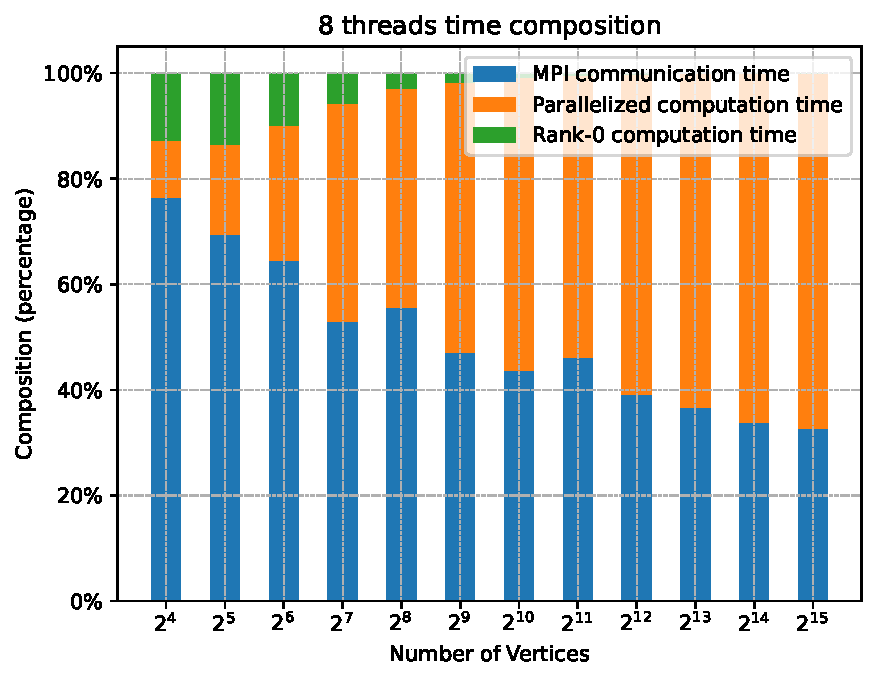
\includegraphics[height=50mm]{mpi_composition_n1_t8.pdf}
			\caption{8 threads time composition}
			\label{fig:mpi_composition_n1_t8}
	\end{subfigure}
	\begin{subfigure}[b]{0.45\textwidth}
		\centering
		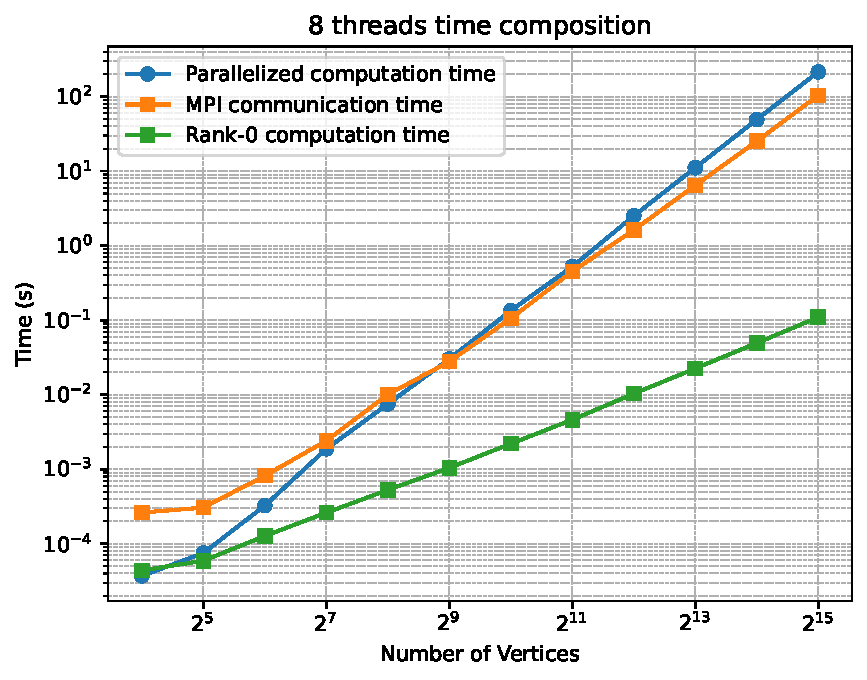
\includegraphics[height=50mm]{time_n1_t8_composition_time.pdf}
		\caption{8 threads time}
		\label{fig:mpi_n1_t8_time}
	\end{subfigure}
	\vspace{0mm} % Space between rows
	% Bottom row, left (c)
	\begin{subfigure}[b]{0.45\textwidth}
			\centering
			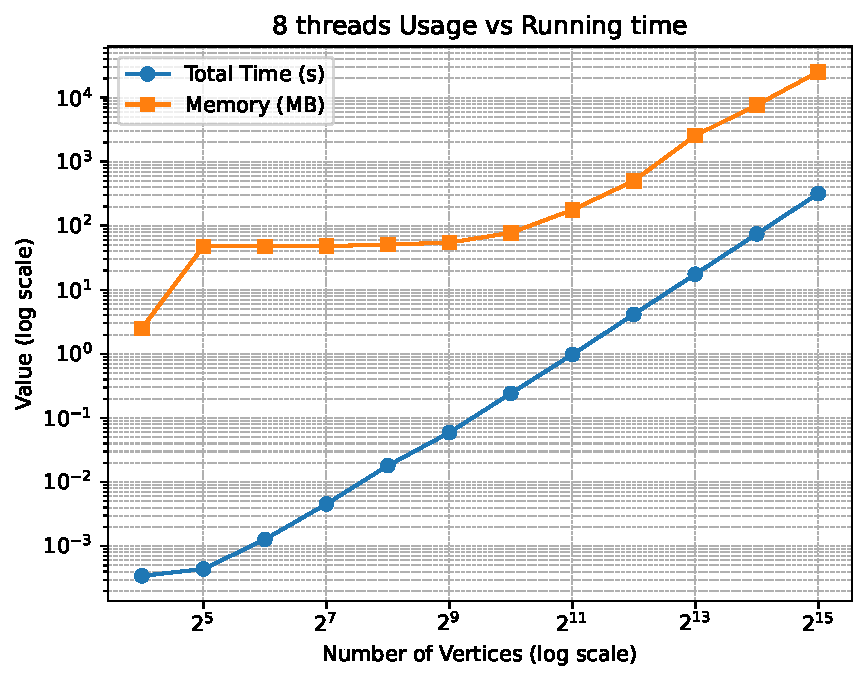
\includegraphics[height=50mm]{time_mem_n1_t8.pdf}
			\caption{8 threads time and memory usage}
			\label{fig:mpi_composition_n1_t8_time_mem}
	\end{subfigure}
	\hfill
	\begin{subfigure}[b]{0.45\textwidth}
		\centering
		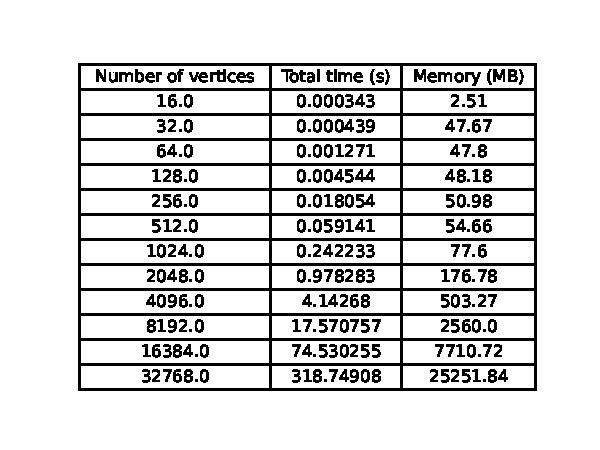
\includegraphics[height=50mm]{time_mem_n1_t8_table.pdf}
		\caption{8 threads time and memory usage table}
		\label{fig:mpi_composition_n1_t8_time_mem_table}
	\end{subfigure}

	\caption{\mstalgo{} with 8 threads}
	\label{fig:mpi_composition_n1_t8_}
\end{figure}

% Composition
% TODO insert round numbers
As the number of vertices per rank increases, the number of rounds grows as predicted by $O(\log{\log(n)})$. However, the runtime does not benefit significantly from the slower round growth, as shown in \cref{fig:mpi_composition_n1_t8_time_mem} and \cref{fig:mpi_composition_n1_t8_time_mem_table}.

When there are only one or a few vertices assigned to each Slurm task, as predicted by the Congested Clique model, the communication time constitutes the majority of the total runtime. Additionally, the rank-0 computation time accounts for a significant fraction of the total runtime, meaning that at least $10\%$ of the time, all other tasks remain idle, waiting for rank-0 to complete its computation. However, as we process larger and larger graphs, the communication time is no longer the dominant factor. Instead, the parallelized computation time starts to dominate, while the rank-0 computation time diminishes, as shown in \cref{fig:mpi_composition_n1_t8}.

% explain why parallelized computation time increases
The parallelized computation time includes all operations other than communication and rank-0 computation. Calculating the minimum-weight edges is a memory-bound task and constitutes a significant portion of the parallelized computation time. The memory required for the graph grows quadratically with the number of vertices, which means the time spent preparing MPI messages also grows accordingly. Further optimization of this algorithm would require more memory-efficient data structures.

In the $2^{15}$-vertex example, the expected memory usage is $2^{15} \times 2^{15} \times 4 = 2^{31}$ bytes = $4096$ MB (assuming double precision). However, the actual memory usage is $25251$ MB, indicating that the message buffers consume the majority of the memory.

% Strong scaling
\begin{figure}[h]
	\begin{subfigure}[b]{0.45\textwidth}
		\centering
		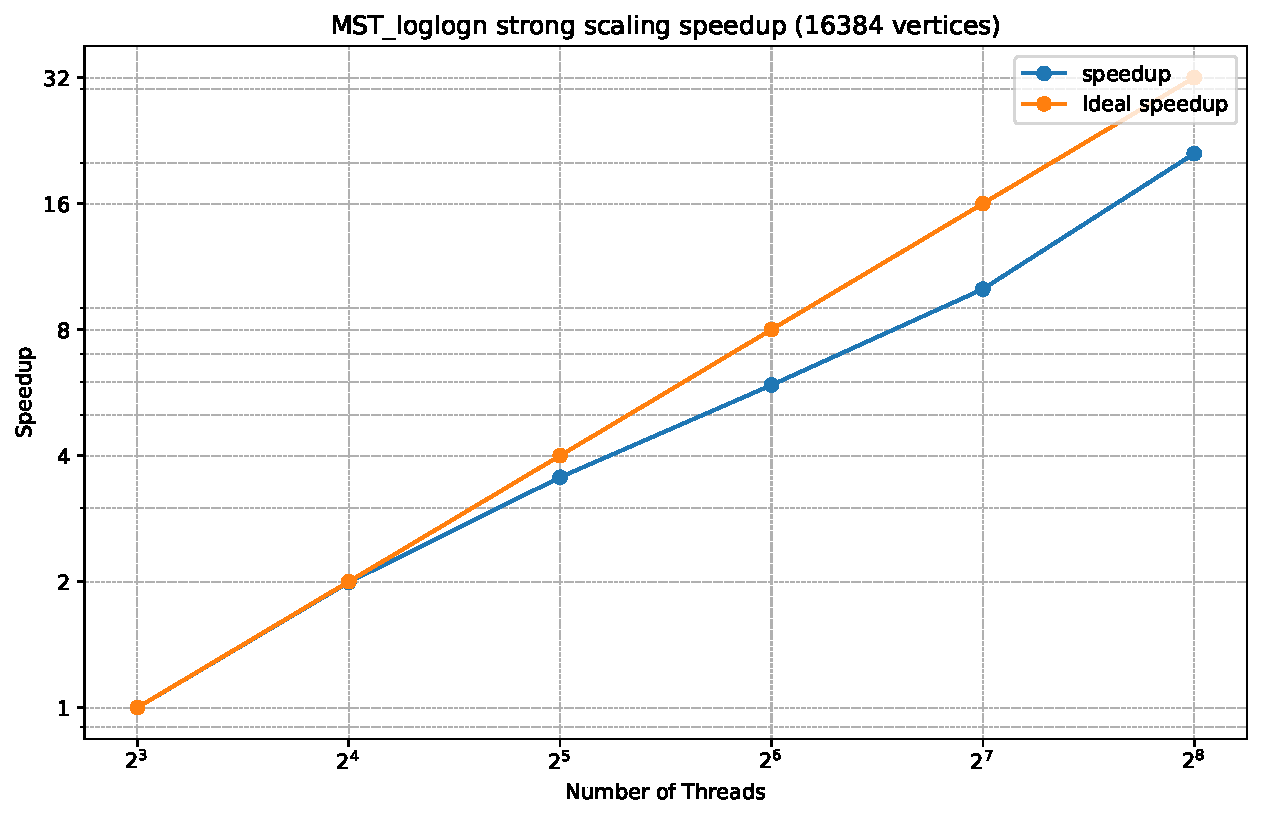
\includegraphics[height=40mm]{strong_scale_16384_speedup.pdf}
		\caption{16384 vertices strong scaling speedup}
		\label{fig:mpi_composition_strong_scaling_16384_speedup}
	\end{subfigure}
	\begin{subfigure}[b]{0.45\textwidth}
		\centering
		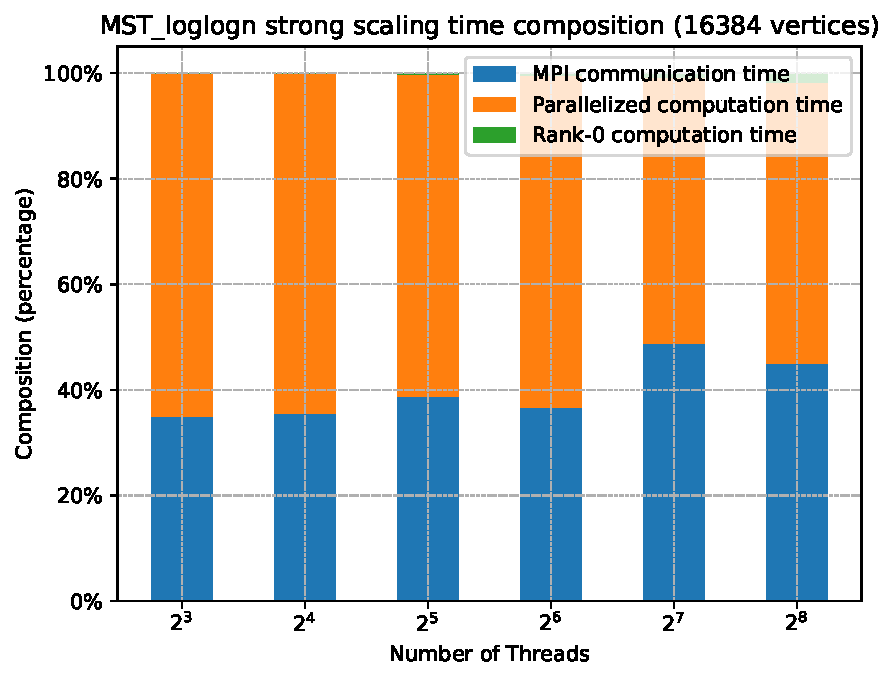
\includegraphics[height=50mm]{strong_scale_16384_composition.pdf}
		\caption{16384 vertices strong scaling time composition}
		\label{fig:mpi_composition_strong_scaling_16384}
	\end{subfigure}
	\vspace{0mm} % Space between rows
	% Bottom row, left (c)
	\begin{subfigure}[b]{1\textwidth}
		\centering
		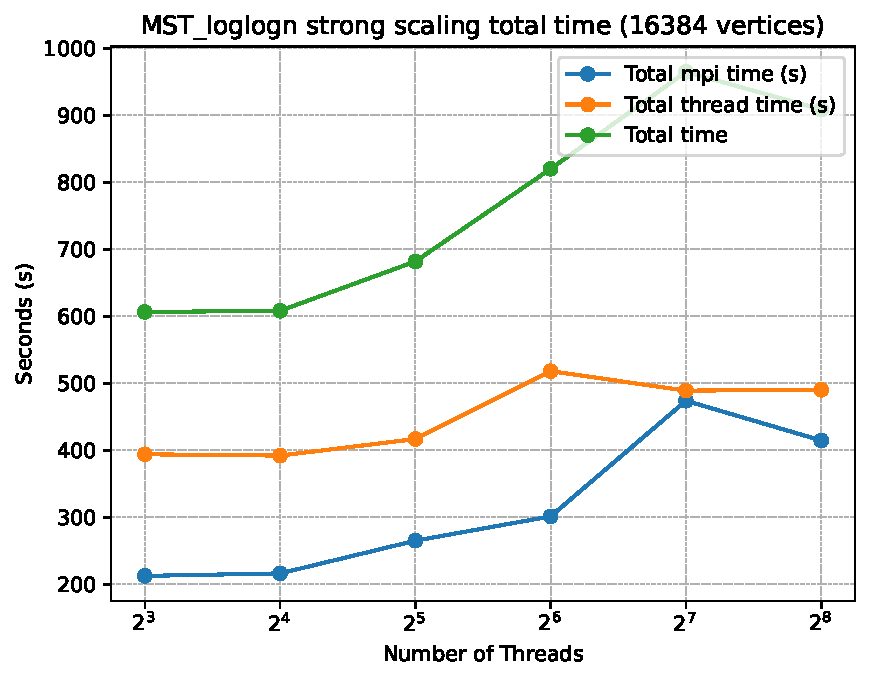
\includegraphics[height=50mm]{strong_scale_16384_total_time.pdf}
		\caption{16384 vertices strong scaling total time}
		\label{fig:mpi_composition_strong_scaling_16384_total}
	\end{subfigure}
	\label{fig:mpi_composition_strong_scaling_16384_}
\end{figure}

We measure the strong scaling performance of \mstalgo{} on Puhti with 16384 vertices and up to 512 Slurm tasks (as provided by Puhti).

The speedup shown in Figure \cref{fig:mpi_composition_strong_scaling_16384_speedup} demonstrates good scalability. It closely follows the ideal speedup line. With 512 tasks, the algorithm achieves a speedup of over 32 compared to the optimal speedup of 64. The parallelized computation time decreases as the number of tasks increases, while the communication and rank-0 computation times grow.

\begin{tcolorbox}[colback=white,colframe=black,boxrule=1pt,arc=0pt]
	Key observation: Compute and communication trade-off. For the same-sized graph, more tasks result in less parallelized computation time (fraction) per task (as it is averaged out) but more communication time (fraction). Vice versa.
\end{tcolorbox}

Figure \cref{fig:mpi_composition_strong_scaling_16384_total} demonstrates that MPI communication time is the major contributor to the slowdown in speedup. When vertices are partitioned, multiple vertices (nodes in Congested Clique terminology) are assigned to the same task. Within each group of vertices, no MPI communication is required. By increasing the number of tasks and further partitioning the vertices, the size of these local groups decreases, resulting in a higher total communication overhead. This explains the poor scalability of MPI communication time in the graphs.

On the other hand, the parallelized computation time shows excellent scalability. The total parallelized computation time remains relatively flat in Figure \cref{fig:mpi_composition_strong_scaling_16384_total}.

If more tasks were available, there would likely be a turning point in speedup where the communication overhead outweighs the benefits of additional tasks. However, due to the limited number of tasks, we cannot reach that point. Nonetheless, \mstalgo{} demonstrates good scalability with the available number of tasks and excellent compatibility with vertex partitioning.

\begin{figure}[h]
	\centering
		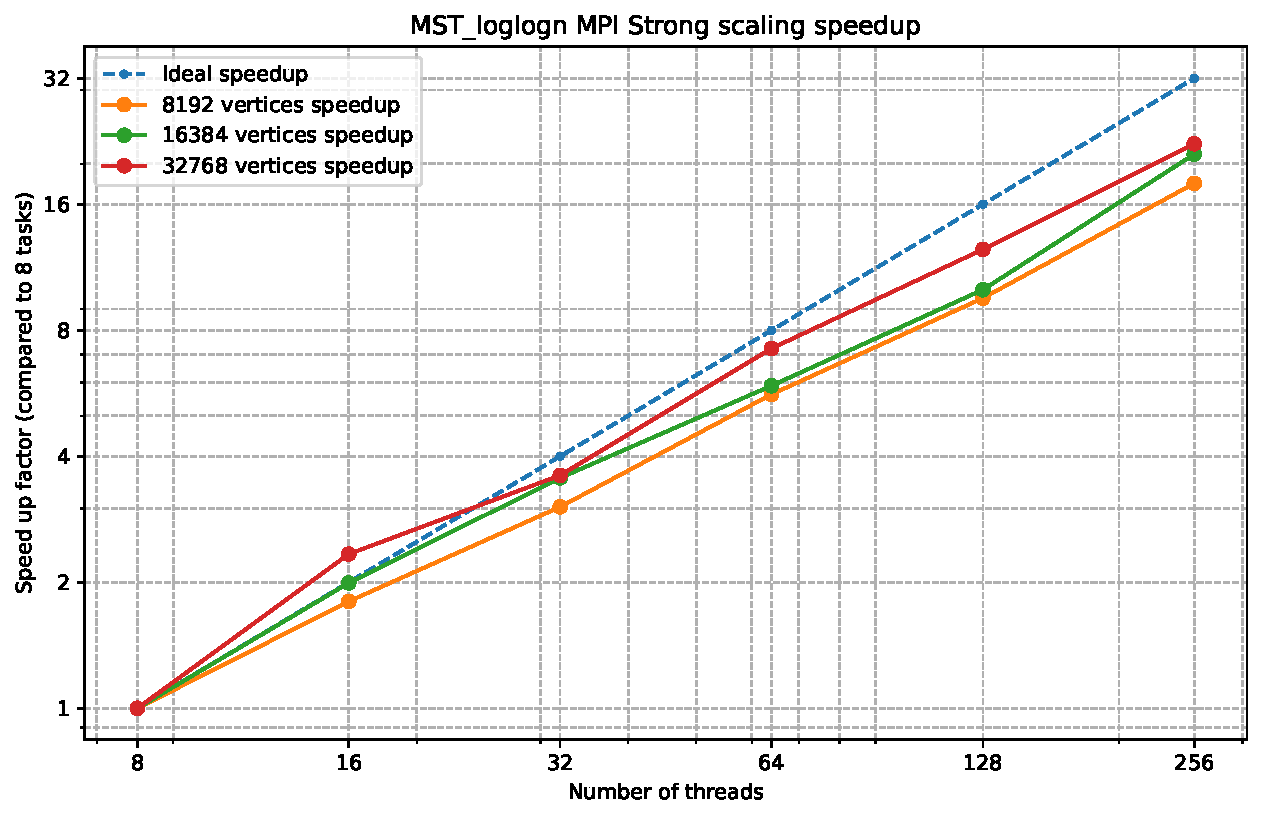
\includegraphics[height=70mm]{mpi_cpp_strong_scaling.pdf}
	\caption{Strong scaling performance of \mstalgo{}}
	\label{fig:mpi_cpp_strong_scaling}
\end{figure}

Figure \cref{fig:mpi_cpp_strong_scaling} illustrates the strong scaling performance of \mstalgo{}. The plot includes three lines corresponding to graphs with \(2^{13}\), \(2^{14}\), and \(2^{15}\) vertices. The number of tasks increases horizontally from 8 to 256.

All three strong scaling plots closely follow the ideal speedup line, indicating that the parallelized computation time dominates the algorithm's execution time \cite{HPCScaling}. Among the three cases, the algorithm scales best with \(2^{15}\) vertices, as its speedup curve is closest to the ideal speedup line. Conversely, the algorithm scales worst with \(2^{13}\) vertices, as its speedup curve deviates the most from the ideal speedup line.

From Figure \cref{fig:mpi_cpp_strong_scaling}, it is evident that larger graphs achieve better speedup with the same number of Slurm tasks. This observation aligns with the time composition shown in Figure \cref{fig:mpi_composition_n1_t8}. For a fixed number of tasks, increasing the number of vertices per task results in more time spent on parallelized computation and less time on MPI communication and rank-0 computation.


% % For capacity and the time composition change between thread counts
% \begin{figure}[h]
% 	\centering
% 	% Top row, left (a)
% 	\begin{subfigure}[b]{0.45\textwidth}
% 			\centering
% 			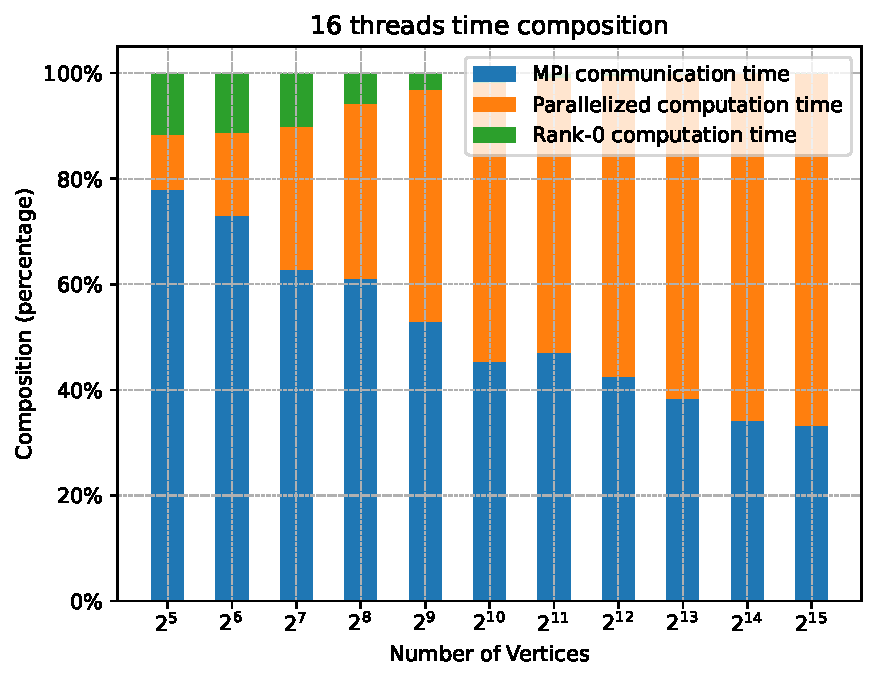
\includegraphics[height=50mm]{mpi_composition_n1_t16.pdf}
% 			\caption{16 tasks time composition}
% 			\label{fig:mpi_composition_n1_t16}
% 	\end{subfigure}
% 	\hfill
% 	% Top row, right (b)
% 	\begin{subfigure}[b]{0.45\textwidth}
% 			\centering
% 			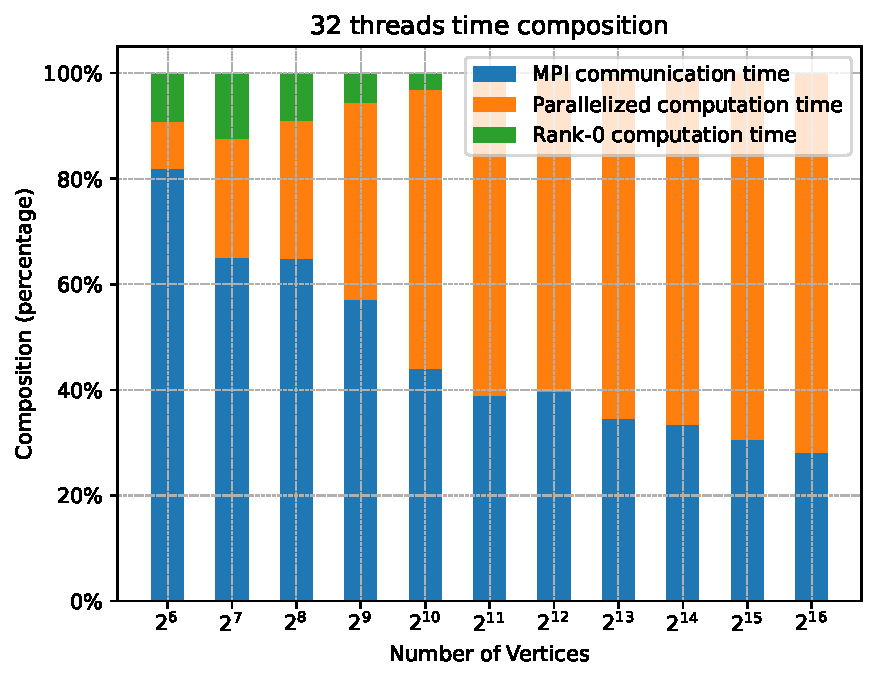
\includegraphics[height=50mm]{mpi_composition_n2_t16.pdf}
% 			\caption{32 tasks time composition}
% 			\label{fig:mpi_composition_n2_t16}
% 	\end{subfigure}
% 	\vspace{0mm} % Space between rows
% 	% Bottom row, left (c)
% 	\begin{subfigure}[b]{0.45\textwidth}
% 			\centering
% 			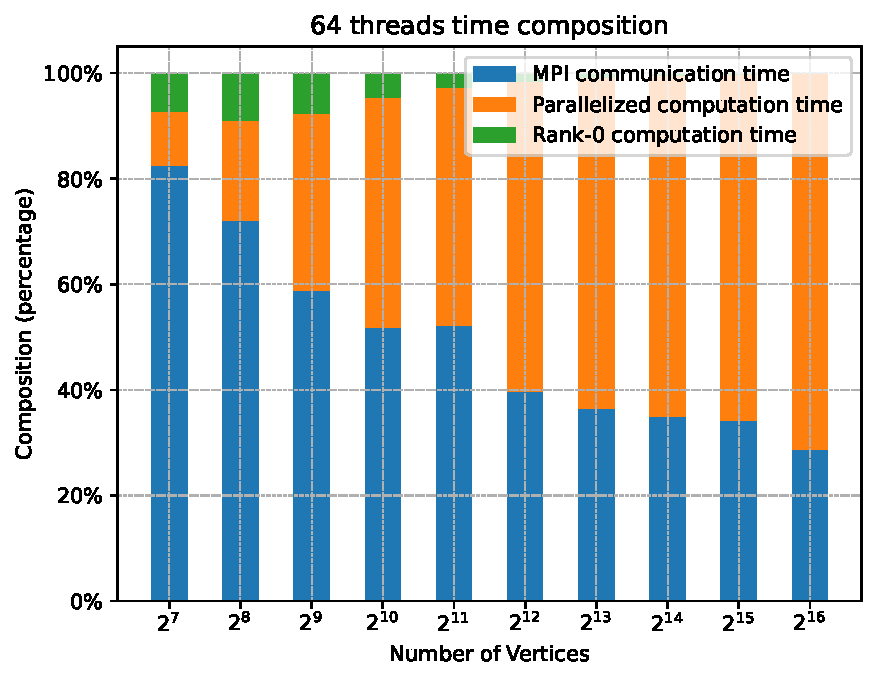
\includegraphics[height=50mm]{mpi_composition_n4_t16.pdf}
% 			\caption{64 tasks time composition}
% 			\label{fig:mpi_composition_n4_t16}
% 	\end{subfigure}
% 	\hfill
% 	% Bottom row, right (d)
% 	\begin{subfigure}[b]{0.45\textwidth}
% 			\centering
% 			\includegraphics[height=50mm]{mpi_num_tasks_fraction.pdf}
% 			\caption{MPI task time composition with varying number of tasks}
% 			\label{fig:mpi_num_tasks_fraction}
% 	\end{subfigure}
% 	\caption{\textit{MST} log-log $n$ time composition with more processes}
% 	\label{fig:mpi_composition_grid}
% \end{figure}

% \begin{figure}[h]
% 	\centering
% 		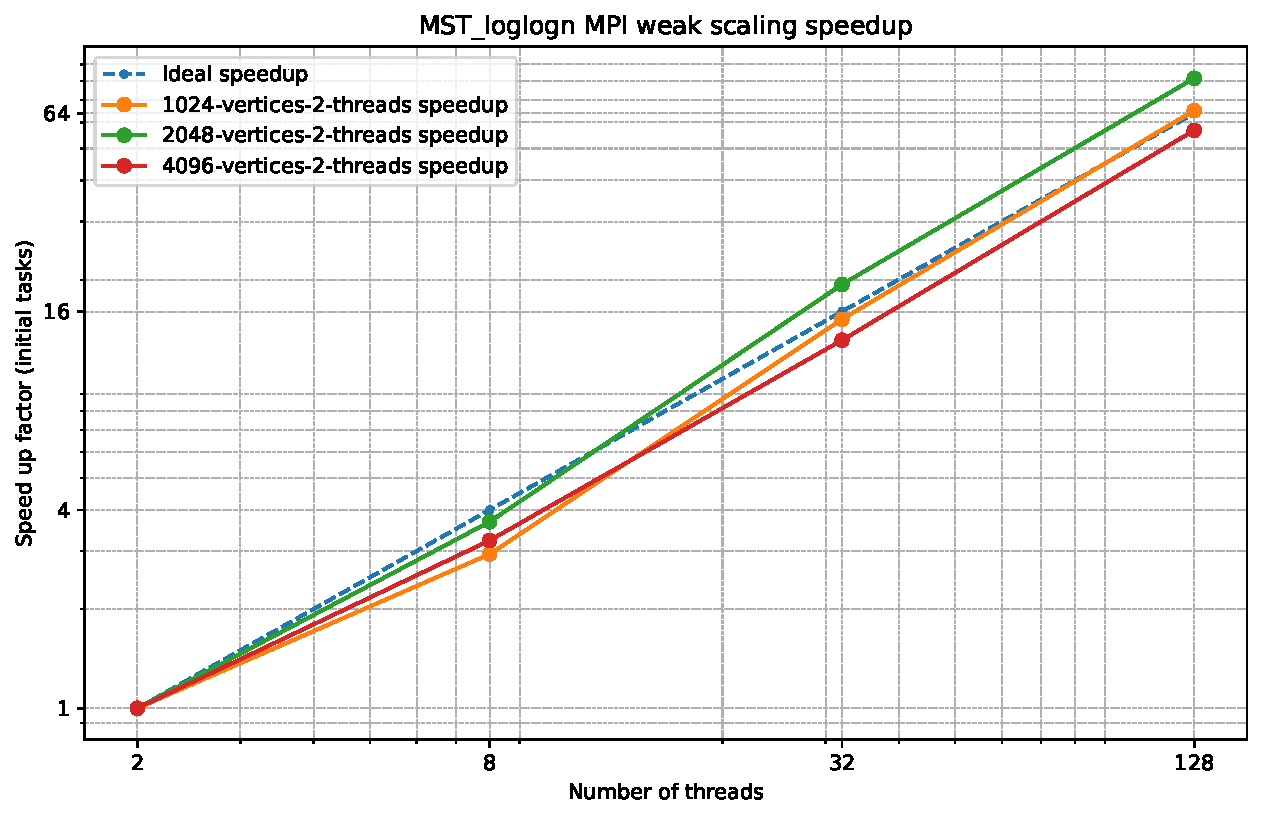
\includegraphics[height=70mm]{mpi_cpp_weak_scaling.pdf}
% 	\caption{Weak scaling performance of \mstalgo{}}
% 	\label{fig:mpi_cpp_weak_scaling}
% \end{figure}

\subsection{Comparison with prim's algorithm}
\begin{figure}[h]
	\centering
		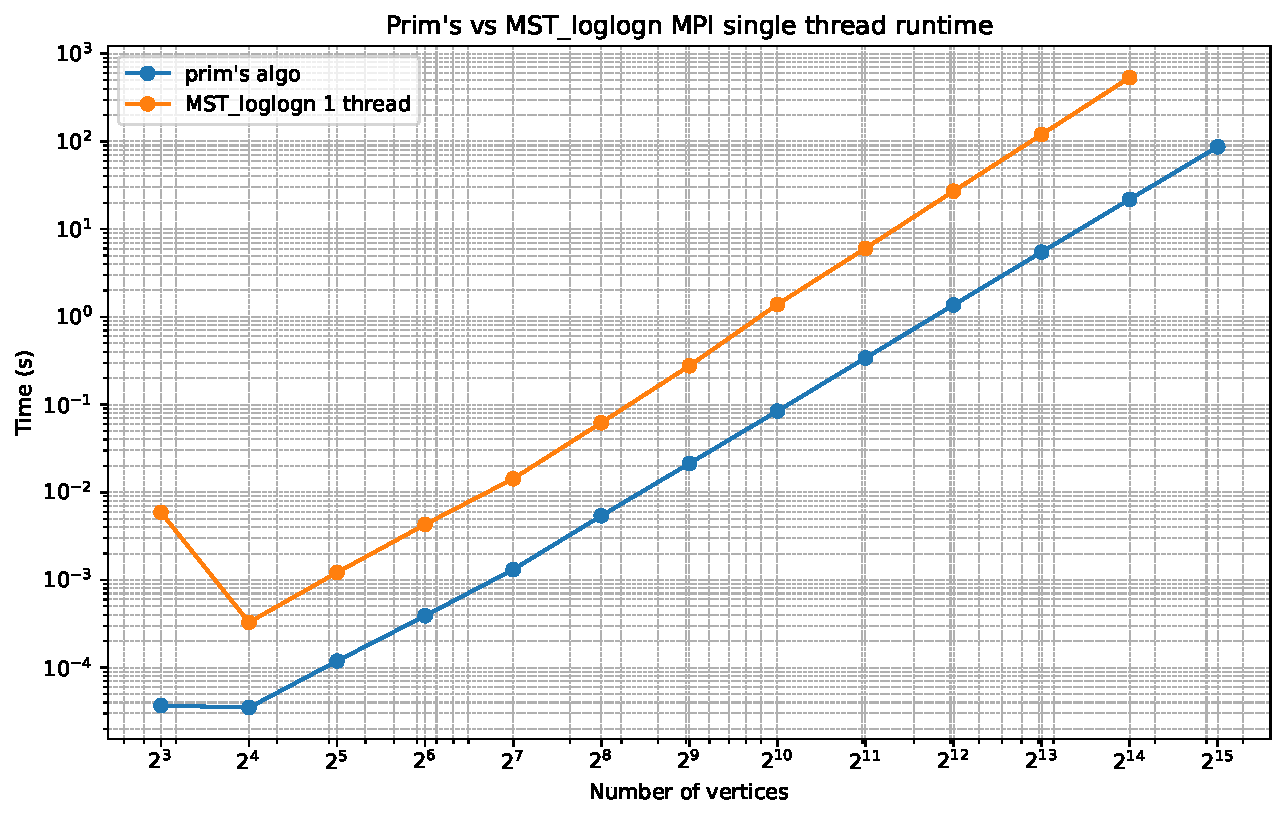
\includegraphics[height=70mm]{prim's_vs_MST_loglogn.pdf}
	\caption{Prim's algorithm compared to \mstalgo{} performance}
	\label{fig:prims_vs_MST_loglogn}
\end{figure}
Prim's algorithm is used as the sequential algorithm to compare the performance of \mstalgo{}. It is implemented in C++ and runs on a single (Slurm) task on Puhti, with 16 GiB of memory.

With 16 GiB of memory, Prim's algorithm can process complete graphs with up to \(2^{15}\) vertices (but not \(2^{16}\)), which corresponds to \(\frac{2^{15} \times (2^{15} - 1)}{2} = 5.33 \times 10^8\) edges, completing in 88 seconds. The bottleneck for Prim's algorithm is the inability to fit larger graphs into the limited memory of a single node.

In contrast, due to the distributed nature of \mstalgo{}, larger graphs can be processed as the number of tasks increases. However, when working on graphs of the same size, \mstalgo{} requires more memory than Prim's algorithm due to the additional memory needed for MPI buffers.

As shown in \cref{fig:prims_vs_MST_loglogn}, with more than 16 tasks, \mstalgo{} is capable of processing complete graphs with up to \(2^{16}\) vertices (but not \(2^{17}\)). Furthermore, \mstalgo{} outperforms Prim's algorithm in terms of speed when there are more than 64 tasks.

\begin{figure}[h]
	\centering
		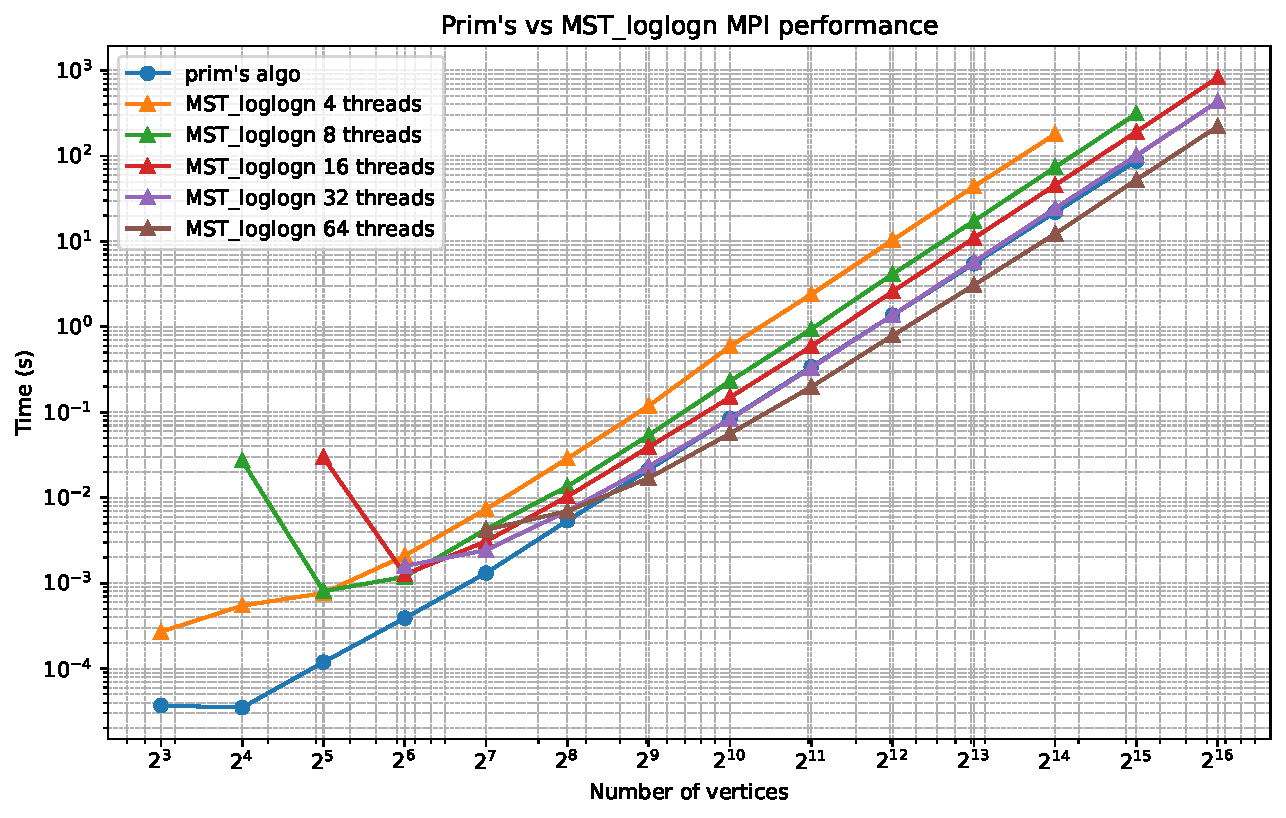
\includegraphics[height=70mm]{prim's_vs_MST_loglogn_single_thread.pdf}
	\caption{Prim's algorithm compared to \mstalgo{} performance with single thread}
	\label{fig:prim's_vs_A_single_thread.pdf}
\end{figure}

When both the prim's algorithm and \mstalgo{} are run on a single thread, the prim's algorithm outperforms \mstalgo{}. The prim's algorithm is more memory efficient and has less computation time. Within the range of the graph size of our work, we see only a minor difference in the time complexity of the two algorithms.
% how well it scales with the number of nodes
% Questioning the time complexity
% bandwidth and optimization
\subsection{Python vs C++}


\begin{figure}[h]
	\centering
		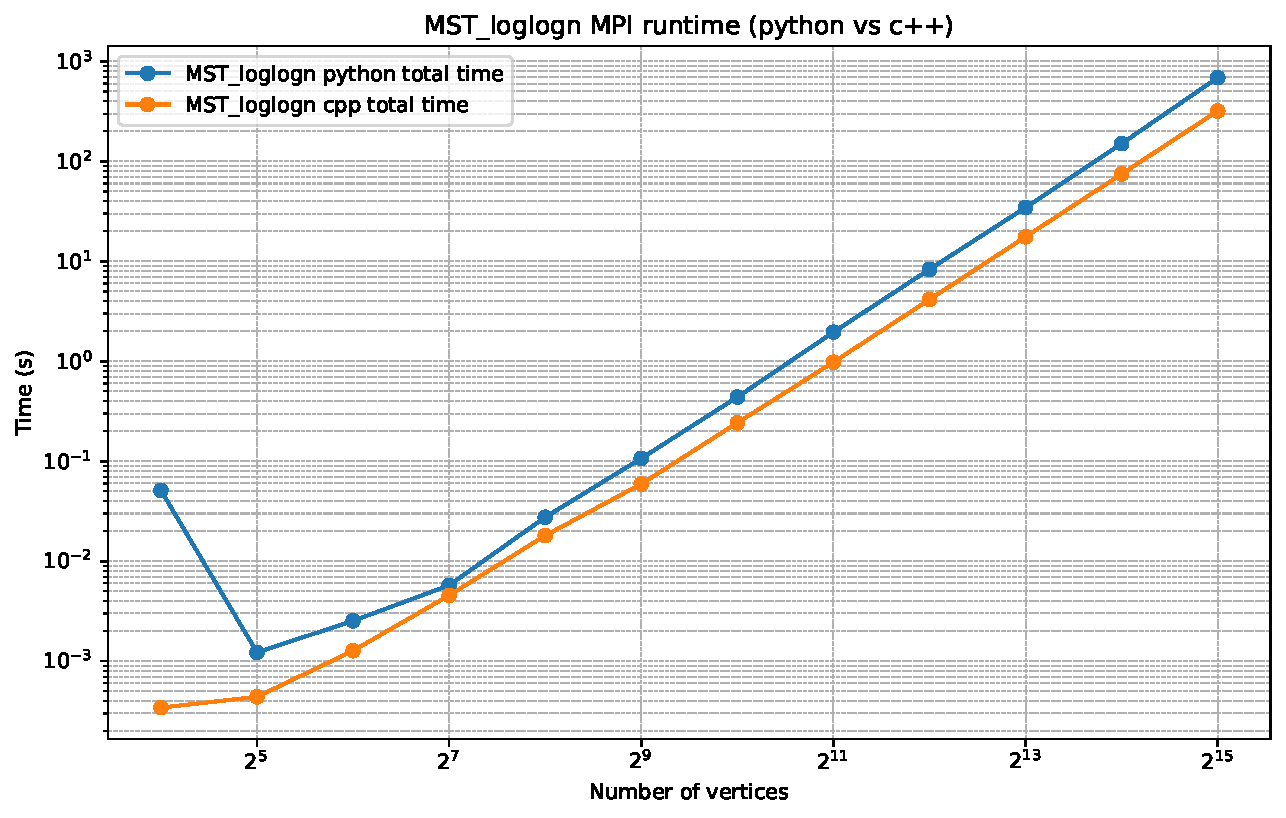
\includegraphics[height=70mm]{n1_t8_cpp_vs_python_total.pdf}
	\caption{\mstalgo{} Python vs C++ time total time}
	\label{fig:python_cpp_mpi_total.pdf}
\end{figure}

\begin{figure}[h]
	\centering
		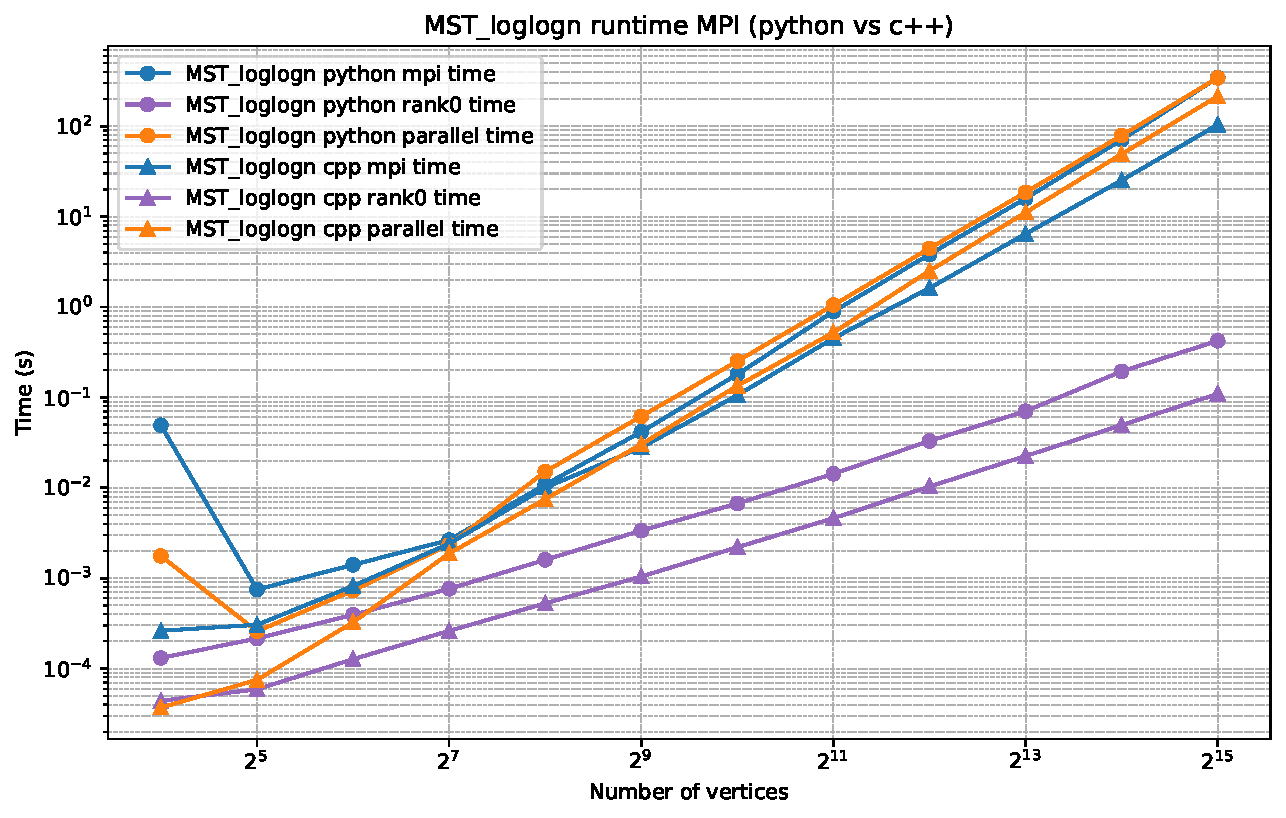
\includegraphics[height=70mm]{n1_t8_cpp_vs_python_composition.pdf}
	\caption{\mstalgo{} Python vs C++ time composition}
	\label{fig:python_cpp_mpi.pdf}
\end{figure}

The runtime difference between the C++ and Python implementations is significant. The slowdown in the Python implementation is primarily due to the memory usage of Python objects, which increases the time required for MPI communication and data processing during computation.

When sending messages with MPI, the data of an edge is encapsulated in an \texttt{Edge} object. This object consists of two integers and a double: the integers represent the origin and destination of the edge, while the double represents the weight of the edge. In Python 3.8.0, an integer object occupies 28 bytes, as indicated by \texttt{sys.getsizeof(int())}. Python integers are instances of the \texttt{PyLongObject} class \cite{PythonInt}, which includes auxiliary fields such as \texttt{ob\_refcnt}, \texttt{ob\_size}, and \texttt{ob\_digit}, leading to their large size. Similarly, a double object in Python occupies 24 bytes. Consequently, the Python \texttt{Edge} object, which combines these components, occupies 80 bytes.

In contrast, the C++ implementation of the \texttt{Edge} object is significantly more memory-efficient. The C++ \texttt{Edge} is implemented as a \texttt{struct} containing two \texttt{int32} integers and a \texttt{float64} double, resulting in a total size of 16 bytes (128 bits). This makes the Python \texttt{Edge} object five times larger than its C++ counterpart.

The larger size of the Python \texttt{Edge} object leads to significantly larger MPI messages, which increases the time spent on MPI communication, as shown in Figure \cref{fig:python_cpp_mpi.pdf}. Additionally, Python incurs more computation overhead compared to C++, further contributing to the slowdown. This is evident in the increased parallelized computation time in Figure \cref{fig:python_cpp_mpi.pdf}.

As a result, the total runtime of the Python implementation is substantially higher than that of the C++ implementation, as demonstrated in Figure \cref{fig:python_cpp_mpi_total.pdf}, despite both implementations using the same algorithm and communication framework.
\clearpage

\section{Congested clique with CUDA}
\label{sec:cuda}
% TODO what is a fair comparison with MPI
GPUs are inherently parallel computing devices and more suitable for parallel computing than CPUs. A Nvidia V100 \cite{PuhtiDoc} has 80 streaming multiprocessors. Each is capable of handing 2048 threads at a time, or 64 warps (with 32 threads each warp) \cite{V100Architecture}. A warp is a group of threads that are executed on a Single Instruction Multiple Thread (SIMT) architecture. The threads in a warp execute the same instruction at the same time but on different data \cite{Simtarch}. Multiple warps can be executed at the same time on a streaming multiprocessor grouped into blocks. A streaming multiprocessor can handle one block at a time or multiple blocks concurrently. This architecture allows Nvidia GPUs to issue a large number of threads and execute them in parallel.

Compared to the CPU, the GPU is a device with more lightweight threads and more parallelism. The number of vertices in a Congested clique is comparable to the number of threads that can be issued on a GPU,
which allows the GPU to simulate a node in the Congested Clique model with a thread.

\cref{alg:mst_cuda} describes the pseudo code of the \mstalgo{} implemented with CUDA, "a general purpose parallel computing platform and programming model that leverages the parallel compute engine in NVIDIA GPUs to solve many complex computational problems in a more efficient way than on a CPU" (\cite{CUDA}).
\subsection{Communication}
\begin{algorithm}
	\caption{\textsc{Minimum Spanning Tree} with CUDA}
	\label{alg:mst_cuda}
	\textbf{Require:} Number of vertices $n$, adjacency matrix $\mathbf{A} \in \mathbb{R}^{n \times n}$.\\
	\textbf{On each thread:} Block index $j$, thread index $i$, block dimension $x$, and adjacency sub-matrix $\mathbf{A}[j \times x + i, :] \in \mathbb{R}^{1 \times n}$.
	\begin{algorithmic}[1]
		\State $v \gets j \times x + i$
		\State $T \gets \emptyset$
		\While{there exists $v \notin T$}
			\If{First phase}
				\State \texttt{speed\_up\_kernel()}
			\Else
				\Comment{Step 1}
				\State \texttt{min\_to\_cluster\_kernel()}
				\Comment{Step 2}
				\State \texttt{min\_from\_cluster\_kernel()}
				\Comment{Step 4}
			\EndIf
			\State Perform \textsc{Construct-Frags} and update $T$
			\Comment{Steps 5 and 6}
		\EndWhile
		\State \textbf{Return} the spanning tree $T$

		\State
		\Function{speed\_up\_kernel()}{}
			\State Find the minimum edge $e(v, v')$ connected to $v$
			\State Write the edge to $v_0$
		\EndFunction

		\State
		\Function{min\_to\_cluster\_kernel()}{}
		\State For each cluster $F' \neq F$, compute $e(v, F') \gets \min_{v' \in F'} \{ e(v, v') \}$.
		\State Write all $e(v, F')$ to leaders $l(F')$
		\EndFunction

		\State
		\Function{min\_from\_cluster\_kernel()}{}
		\State For each cluster $F' \neq F$, compute $e(v, F') \gets \min_{v' \in F'} \{ e(v, v') \}$
		\State Perform \textsc{Cheap-Out} and write the edge $e$ $v_0$
		\EndFunction
	\end{algorithmic}
\end{algorithm}

With CUDA, the computation and communication are handled by kernel functions. Kernels functions are functions that are launched to run on the GPU. The threads lives in the context of kernel function. Each  thread simulates one machine in the Congested Clique model, which is a vertex in the clique graph. Each CUDA thread has its own memory space corresponds to the machine memory in the Congested Clique model.

Threads can write and read from the memory space to achieve communication. When thread $A$ sends a message to thread $B$ in the Congested Clique Model, thread $A$ writes the message to the memory space and thread $B$ reads the message from the memory space.

Each kernel function handles only one communication round. This ensures all the communication rounds are synchronized. We don't need barrier with in the kernel. The kernel function exits when all the threads finish their communication and computation. The result of the kernel function resides in the memory space for communication.

The communication is handled in the following way:
\begin{itemize}
	\item[--] step 1: \texttt{min\_to\_cluster\_kernel}
	\item[--] step 2: \texttt{min\_from\_cluster\_kernel} (comm2)
	\item[--] step 3: Buffers are copied to the host
	\item[--] step 4: CPU computation
	\item[--] step 5: The updated cluster info is copied backed in to the Device memory
	\item[--] step 6: Same as above\
\end{itemize}

There are two kernels in algorithm \cref{alg:mst_cuda}, 
namely \texttt{min\_to\_cluster\_kernel} and \texttt{min\_from\_cluster\_kernel}, corresponding to the first and the second steps in \mstalgo{}. Between the two kernel calls, the buffers are not copied back to the host but are kept in the device memory.

When there is only on machine active in step 3, instead of launching a kernel function with a single thread, that part of the computation is done on the CPU. CPU is far more efficient in handling single-threaded computation than the GPU. Thus, we simply write the edge to the memory space of the machine 0 to simulate the gathering process at step 3. Similarly, step 5 and 6 are done by copying the updated cluster information back to the device memory.

\subsection{Memory read and write}
Threads communicate with each other by reading and writing into the vram of V100. When thread $A$ sends a message to thread $B$, thread $A$. For the correctness of the communication, we eliminate the data race scenarios where multiple threads write to the same memory space e.g. when thread $A$ and thread $C$ all send a message to thread $B$.

Two pointers are passed as input arguments into the first kernel \texttt{min\_to\_cluster\_kernel}: \texttt{min\_edges\_bufGPU}, which has all the graph edges with shape $n \times n$ and \texttt{to\_cluster\_bufGPU}, which is the output of the kernel with shape also $n \times n$, where $n$ is the number of vertices in the complete graph. When thread $A$ sends a message to the leader of cluster $F$, it writes the edge to \texttt{to\_cluster\_bufGPU} $[A, leader(F)]$. There are at least $n$ clusters in the graph, so $leader(F)$ never overflows the buffer. One thread send at most one edge to another cluster leader, so each entry in the buffer is a unique space analogous to a link in the Congested Clique model.

With the second kernel \texttt{min\_from\_cluster\_kernel}, two pointers \texttt{to\_cluster\_bufGPU} and \texttt{from\_cluster\_bufGPU} are passed as input arguments. Among them, \texttt{from\_cluster\_bufGPU} is the output of the kernel. It is another $n$ by $n$ buffer. Because at the end of this stage, one cluster will not send more edges than the number of member of the cluster to vertex $0$. There will be at most $n \times n$ edges sent to vertex $0$.

The space of \texttt{from\_cluster\_buf} is arranged in the following way. Each cluster will gets a \texttt{start\_idx} and an \texttt{end\_idx} to indicate the space allocated to the cluster in the array. \texttt{start\_idx} $-$ \texttt{end\_idx} is the number of vertices in the cluster. The \texttt{end\_idx} of cluster $F$ is the same as the \texttt{start\_idx} of cluster $F+1$, making sure the space is not overlapped. This makes up the space for the edges sent to vertex $0$ with the size of maximum $n \times n$.

Finally, rank $0$ or the CPU reads the buffer \texttt{from\_cluster\_buf} and filters out all the edges not \texttt{null} and continues to perform \texttt{Construct-Frags}.

\subsection{Complete and sparse graphs}
% Why sparse graph
The Nvidia V100 GPU has the capability to issue a huge amount of threads but with a limited VRAM of $16G$ / $32G$. The total memory can be used is much lower than the previous MPI simulation of $8G$ / $16G$ per thread. Compared to the MPI implementation, V100 can only store much less edges in the memory, even it has the capability to launch a large quantity of threads for vertices. A V100 can issue $2048$ threads on each streaming multiprocessor, which is $80 \times 2048 = 163840$ threads in total. We walk around this limitation by introducing sparse graphs. Sparse graphs saturate the GPU's thread capability better by having less edges on each vertex. In this way, the computation is better balanced among the threads.

In the Congested Clique, the network graph is the equivalent as the graph to be solved, which is a complete graph / network. Each vertex / thread, has a list of weight of adjacent edges in memory. In the sparse graph setting, each vertex has a varying number of adjacent edges. The edges of the graph are represented as a adjacent list when generated. The network remains fully connected in the sparse graph setting, meaning any thread and send message to any other threads.

\mstalgo{} works on the sparse graph as well.
% adjacency list/matrix
In memory, a complete graph is represented by an adjacency matrix, where each column represents the adjacent edges of a vertex. Whereas the sparse graph is represented by an adjacency list due to the varying rank of each vertex. Each vertex has a list of adjacent edges.

% Why the algo works on sparse graph
\begin{tcolorbox}[colback=white,colframe=black,boxrule=1pt,arc=0pt]
	\mstalgo{} is designed to work on a complete graph but it does work for connected spares graphs as well.

	\textbf{Proof}: A sparse graph $G$ is analogous to a complete graph $G'$ with weight of edges which are disconnected in the sparse graph set to infinity. \mstalgo{} is capable of finding the MST in $G'$. The edges with infinite weight will not be picked in step 4 for $G'$, meaning they can be removed from the candidate list of step 4. Same for the previous steps. As the network remains fully connected, the infinite weight edges will not affect the communication. Thus, the edges with infinite weight can be ignored in the computation to form a sparse graph.
\end{tcolorbox}

To generate a connected sparse graph, the following steps are taken.
\begin{itemize}
	\item[--] Generate a Prüfer sequence with all the vertices. A Prüfer sequence is an unique sequence of vertices that encodes a tree \cite{Prufer1918}. The tree serves as the skeleton of the sparse graph making sure the graph is connected.
	\item[--] Convert the Prüfer sequence into a tree.
	\item[--] Add edges to the tree randomly until the expected rank is met.
\end{itemize}

\subsection{Best practices}
Similar practices used in the MPI implementation are used on the CUDA implementation to ensure a relatively fair comparison.
% list
\begin{itemize}
	\item[--] The constructed MST is maintained as a union-find data structure.
	\item[--] Same edge objects and weight datatype are used in the CUDA implementation as in the MPI implementation.
	\item[--] The simplification on the first phase is applied.
\end{itemize}

\subsection{Profiling}
To accurately measure the performance of the CUDA implementation, we need to profile the program. The profiling is done with nvprof, a command-line profiler provided by Nvidia. The profiling result shows the time spent on the memory copying and the kernel functions. The time spent on each kernel function is the time spent on the communication and local computation in each round.

\clearpage

\section{Performance with CUDA}
\label{sec:cuda_performance}
\subsection{Conclusion overview}

\begin{itemize}
	\item CUDA implementation of \mstalgo{} demonstrates significant speedup compared to single-threaded Prim's algorithm, leveraging the GPU's parallelism.
	\item The communication between threads is efficiently handled using memory read and write operations, analogous to message passing in the Congested Clique model.
	\item The time spent on kernel execution scales well with the number of vertices, but memory operations and CPU computation become bottlenecks as graph size increases.
	\item Sparse graphs show potential for better workload balancing on GPUs, but the overhead of adjacency list operations can negate performance gains.
	\item Smaller block sizes improve workload distribution among Streaming Multiprocessors (SMs), reducing kernel execution time.
	\item CUDA implementation is limited by GPU memory capacity, making it challenging to handle large complete graphs without sparsity.
\end{itemize}

% 1. How is the read and write analogous to the communication. How much time it takes? Is it the majority of the time? How does divergence affect the performance (Check the assembly maybe)?

% 2. How much time does rank-0 time take compared to the gpu time? Will it become the bottleneck at some point?

% 3. Does sparse graph promote better workload balancing?

% 4. Is it fair to compare with MPI? Can we fit equal large graphs into the memory? MPI vs single V100 why?

% 5. Compared with a single threads Prim's, can we beat it? (Compare the theoretical peak flops and the actual flops, are we utilizing the hardware well?)

% 6. How well does the algorithm scale with the number of threads? (Can we scale further with MPI?) (Optional)

% 1024 / 2048 per block what's the diff.
% What to compare (CPU single thread? why not)
\subsection{Performance}
% TODO 1, 2, 4, 6
\begin{tcolorbox}[colback=white,colframe=black,boxrule=1pt,arc=0pt]
As shown in the figure, DtH refers to the initial data transfer from the host to the device. This operation scales proportionally with the graph size, as the entire graph data must be copied to the GPU memory. Conversely, HtD represents the final data transfer from the device back to the host, which scales at a slower rate due to the reduced amount of data being transferred.

Within the kernels, each thread simulates a machine in the congested clique model. At the beginning of each round, threads are responsible for receiving messages, which corresponds to reading from the buffer. Subsequently, threads process the received data and send their own messages, which involves writing to a new buffer.

The workload on the \texttt{to\_cluster\_kernel} is notably larger than that on the \texttt{from\_cluster\_kernel}. This is because, at the start of the algorithm, there are significantly more edges to process, resulting in a higher computational demand for the \texttt{to\_cluster\_kernel}.
\end{tcolorbox}

\begin{figure}[h]
	\begin{subfigure}[b]{0.45\textwidth}
		\centering
		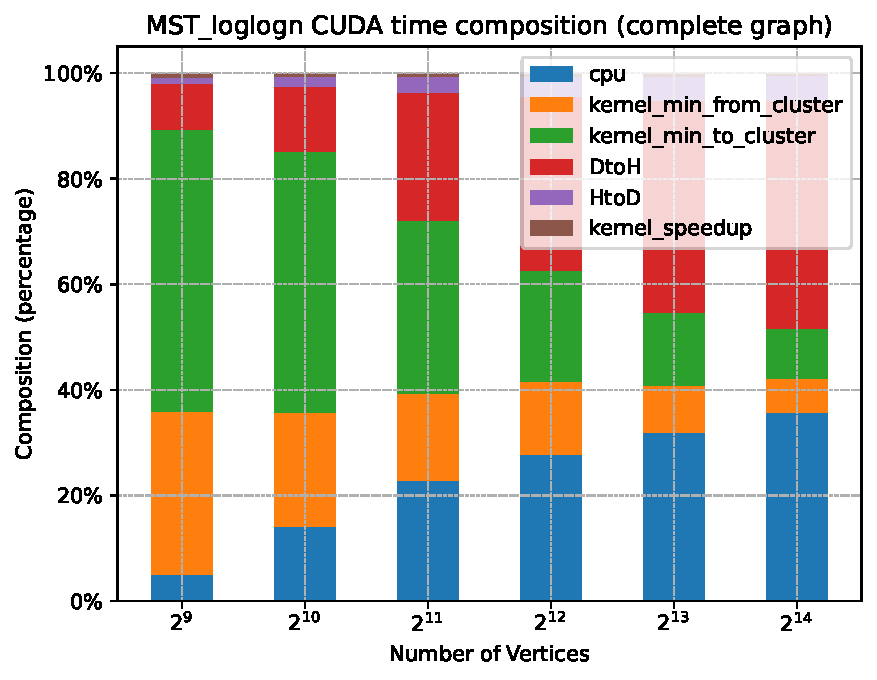
\includegraphics[height=50mm]{cuda_composition_complete.pdf}
		\caption{\mstalgo{} CUDA time composition with complete graph}
		\label{fig:cuda_composition_complete.pdf}
	\end{subfigure}
	\begin{subfigure}[b]{0.45\textwidth}
		\centering
		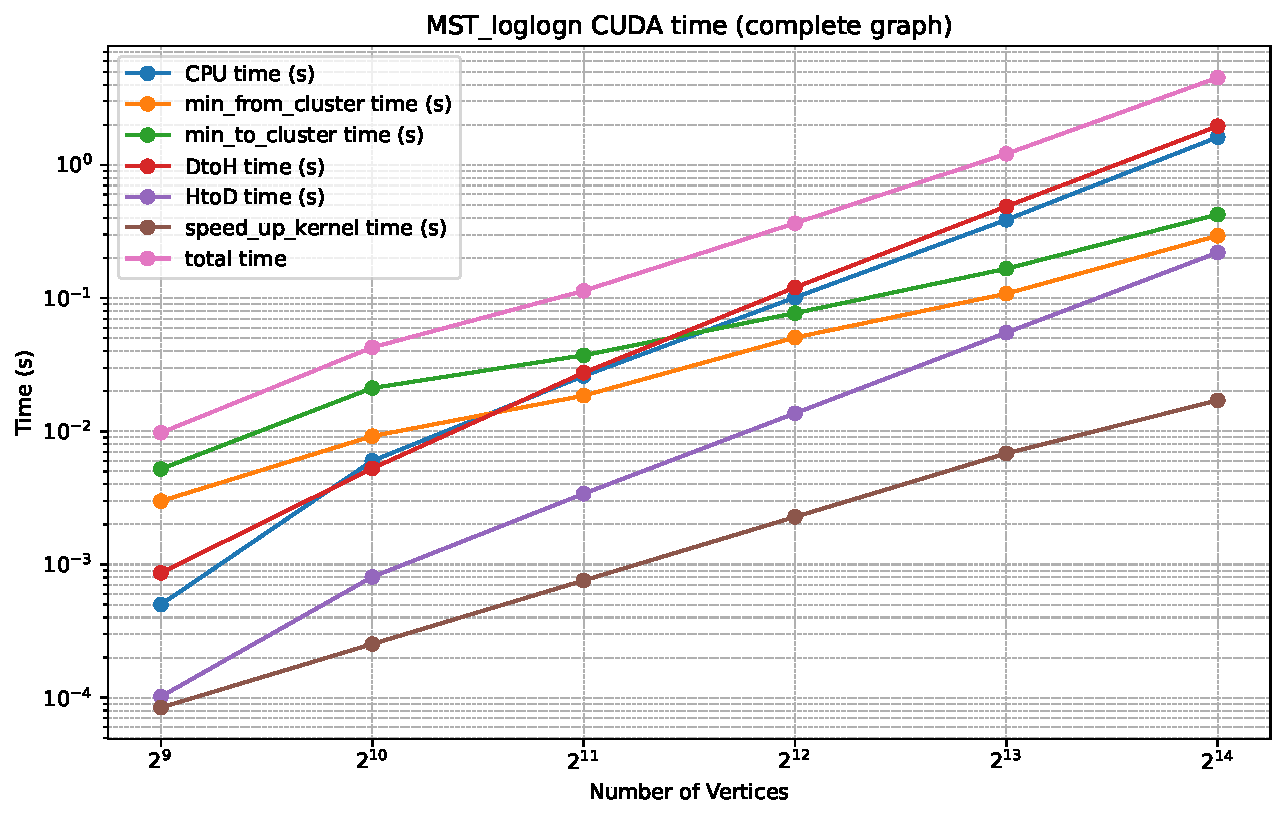
\includegraphics[height=50mm]{cuda_composition_complete_time.pdf}
		\caption{\mstalgo{} CUDA time with complete graph}
		\label{fig:cuda_composition_complete_time.pdf}
	\end{subfigure}
	\caption{\mstalgo{} CUDA time composition with complete graph. Each block has 1024 threads, each thread simulates a vertex.}
	\label{fig:cuda_composition_complete}
\end{figure}

We run the CUDA implementation \cref{alg:mst_cuda} on Puhti with a Nvidia V100 GPU. There are massive amount of thread resources on one V100. The workload of complete graphs are not able to saturate the thread resources before the vram is full. \cref{fig:cuda_composition_complete} shows the time composition and total time of the CUDA implementation with complete graphs. The number of vertices scales from $2^{9}$ to $2^{14}$. Considering the communication buffers used in the program, $2^{14}$ is the largest graph that can be fit into the vram of a V100. The number of threads in each block is $1024$.

Because the maximum amount of threads can be issued is around $2^{26}$ on V100, Every vertices can be mapped to a thread during the scaling. Compared to the $|E|$ of the graph, which scales quadratically with the number of vertices, the workload among the threads scale linearly within the kernel. However, having the workload scales linearly in the kernels doesn't mean it scales linearly throughout.

\cref{fig:cuda_composition_complete_time.pdf} shows the time of each kernel, memory operation, CPU and total time of the program as the number of vertices increases. The time of \texttt{min\_to\_cluster\_kernel} and \texttt{min\_from\_cluster\_kernel} increases noticeably slower compared to other time categories. On contrast, the time of memory operations and CPU computation increases noticeably faster. The workload for them can not be distributed to more work units like with the kernels. Thus they scale corresponds to $|E|$.

% Composition change
From \cref{fig:cuda_composition_complete.pdf}, we see the composition changes during the scaling. As explained earlier, The CPU time and memory copying time remain insignificant when the number of vertices is small, but as the number of vertices increases, these times become more prominent. Eventually, the kernels time is insignificant, and the nonparallelizable part of the program contributes over $80\%$ of the total time, when graph size reaches $2^{14}$ vertices.


\begin{figure}[h]
	\centering
		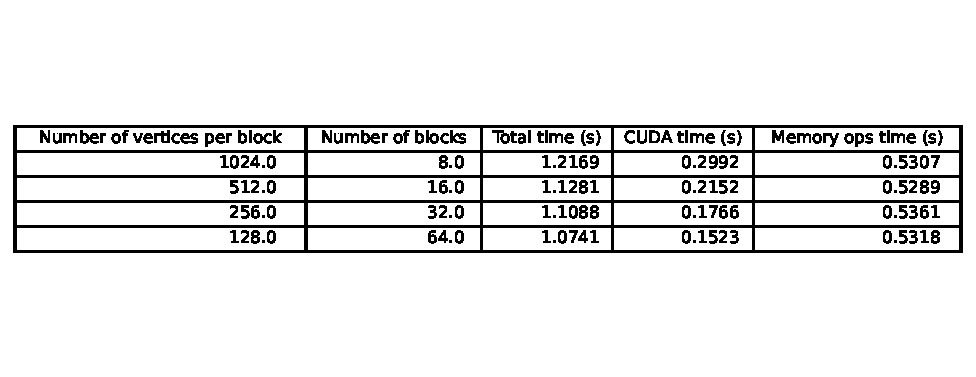
\includegraphics[height=45mm]{cuda_complete_varying_block_size_8192.pdf}
	\caption{\mstalgo{} CUDA time with complete graph with varying block size}
	\label{fig:cuda_complete_varying_block_size_8192.pdf}
\end{figure}

However, the CUDA time can be further reduced by having smaller block sizes, when the SMs are not well saturated. \cref{fig:cuda_complete_varying_block_size_8192.pdf} shows the time of the CUDA implementation with complete graphs with $8192$ vertices and varying block sizes. The number of vertices is fixed to $8192$. The time of the program decreases as the block size decreases. The time of the program is the lowest when the block size is $256$. The time of the program increases when the block size is further decreased.

Going from block size $1024$ to $128$, the CUDA time is reduced almost by half. More blocks are launched with smaller block size, which means more SMs are utilized. The reduction in time is from the less warps on each Streaming Process (SP), going from $32$ to $4$ warps with $32$ threads in each warp. When there are SMs idling, this is a good way balancing the workload among the SMs.

% small conclusion??

\subsection{Complete vs sparse graph}

\begin{figure}[h]
	\begin{subfigure}[b]{0.45\textwidth}
		\centering
		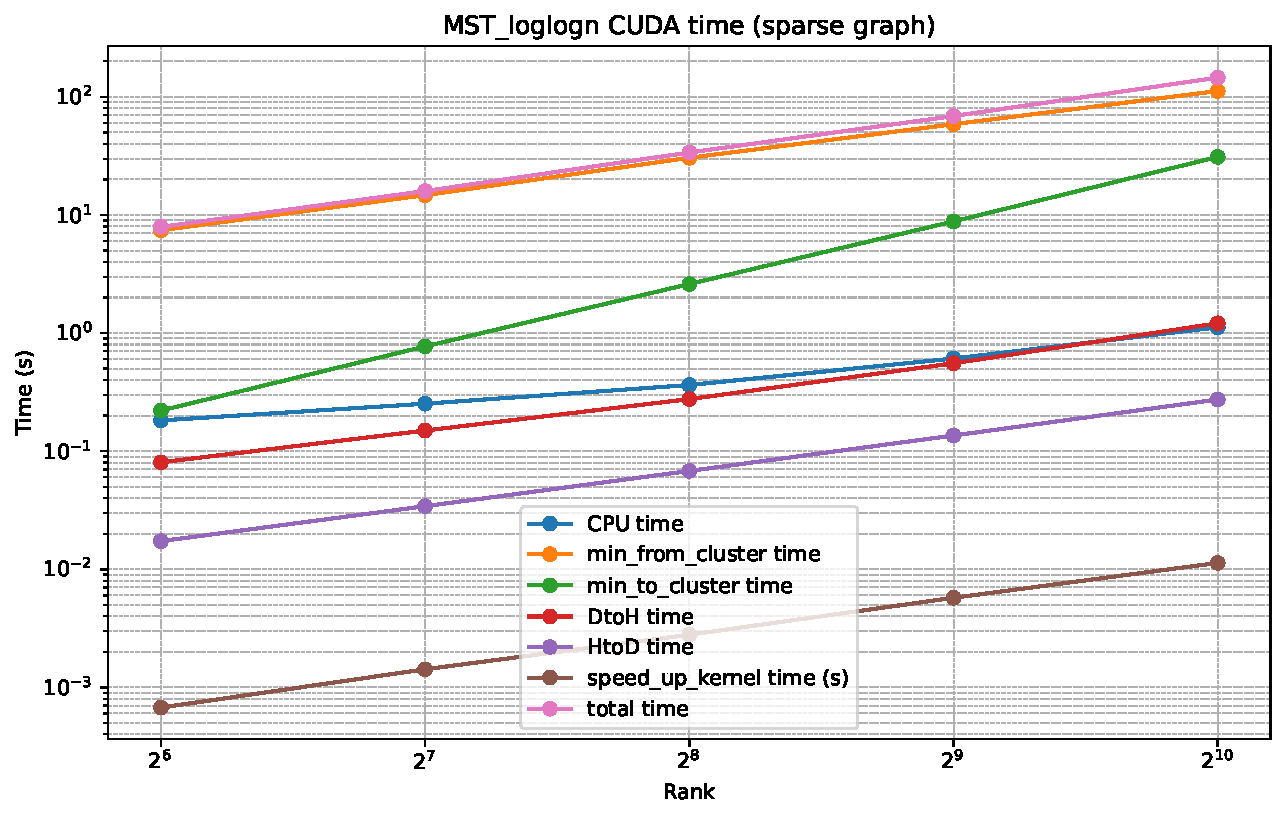
\includegraphics[height=40mm]{cuda_composition_sparse_time.pdf}
		\caption{\mstalgo{} CUDA time composition with sparse graph}
		\label{fig:cuda_composition_sparse_time.pdf}
	\end{subfigure}
	\begin{subfigure}[b]{0.45\textwidth}
		\centering
		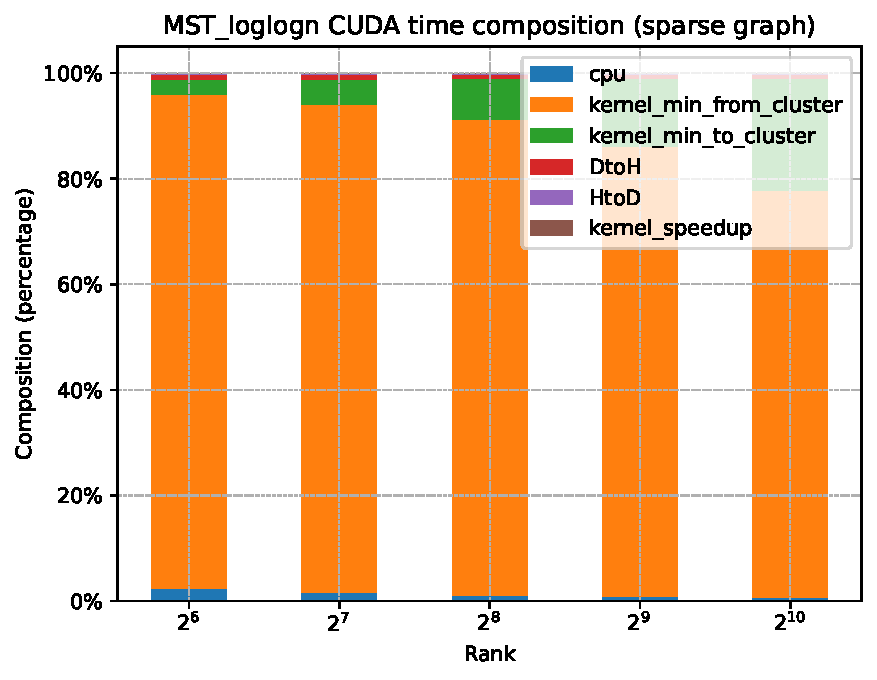
\includegraphics[height=45mm]{cuda_composition_sparse_persistent.pdf}
		\caption{\mstalgo{} CUDA time with complete graph}
		\label{fig:cuda_composition_sparse_persistent.pdf}
	\end{subfigure}
	\caption{\mstalgo{} CUDA time composition with sparse graph. There is a block on each SM and each block has 1024 threads/vertices.}
	\label{fig:cuda_composition_sparse}
\end{figure}

We modified \cref{alg:mst_cuda} to work with sparse graphs. The algorithm itself works out of the box with sparse graph. But the buffer allocation and accessing need to be modified to comply with the sparsity. Each SM possess $1024$ vertices with $1024$ threads, resulting in $80 \times 1024 = 81920$ vertices in total in the sparse graph. \cref{fig:cuda_composition_sparse_time.pdf} shows the time of the CUDA implementation with sparse graphs. The x-axis is the average rank of the sparse graph, which goes from $64$ to $1024$.

However, the time of the CUDA implementation with sparse graphs is even larger than the time of memory operations and CPU computation. Whereas in the complete graphs, the time of the CUDA implementation is smaller than the time of memory operations and CPU computation. This is the exact opposite of the expectation. Most of the slow down is caused by the data structure overhead from the sparse graph. Because of the sparsity of the adjacent list. When you access the adjacent list, you have to loop through all the edges to find the edge to vertex $v$. This is a $O(n)$ operation. The time of the kernel is $O(n^2)$ in the worst case.  And there are more clusters at the beginning which means more workload in the kernel. Thus in \cref{fig:cuda_composition_sparse}, the kernels are taking the most time, and \cref{fig:cuda_composition_sparse} the sparse graph is slower than the complete graph with the same amount of edges.

\begin{figure}[h]
	\centering
		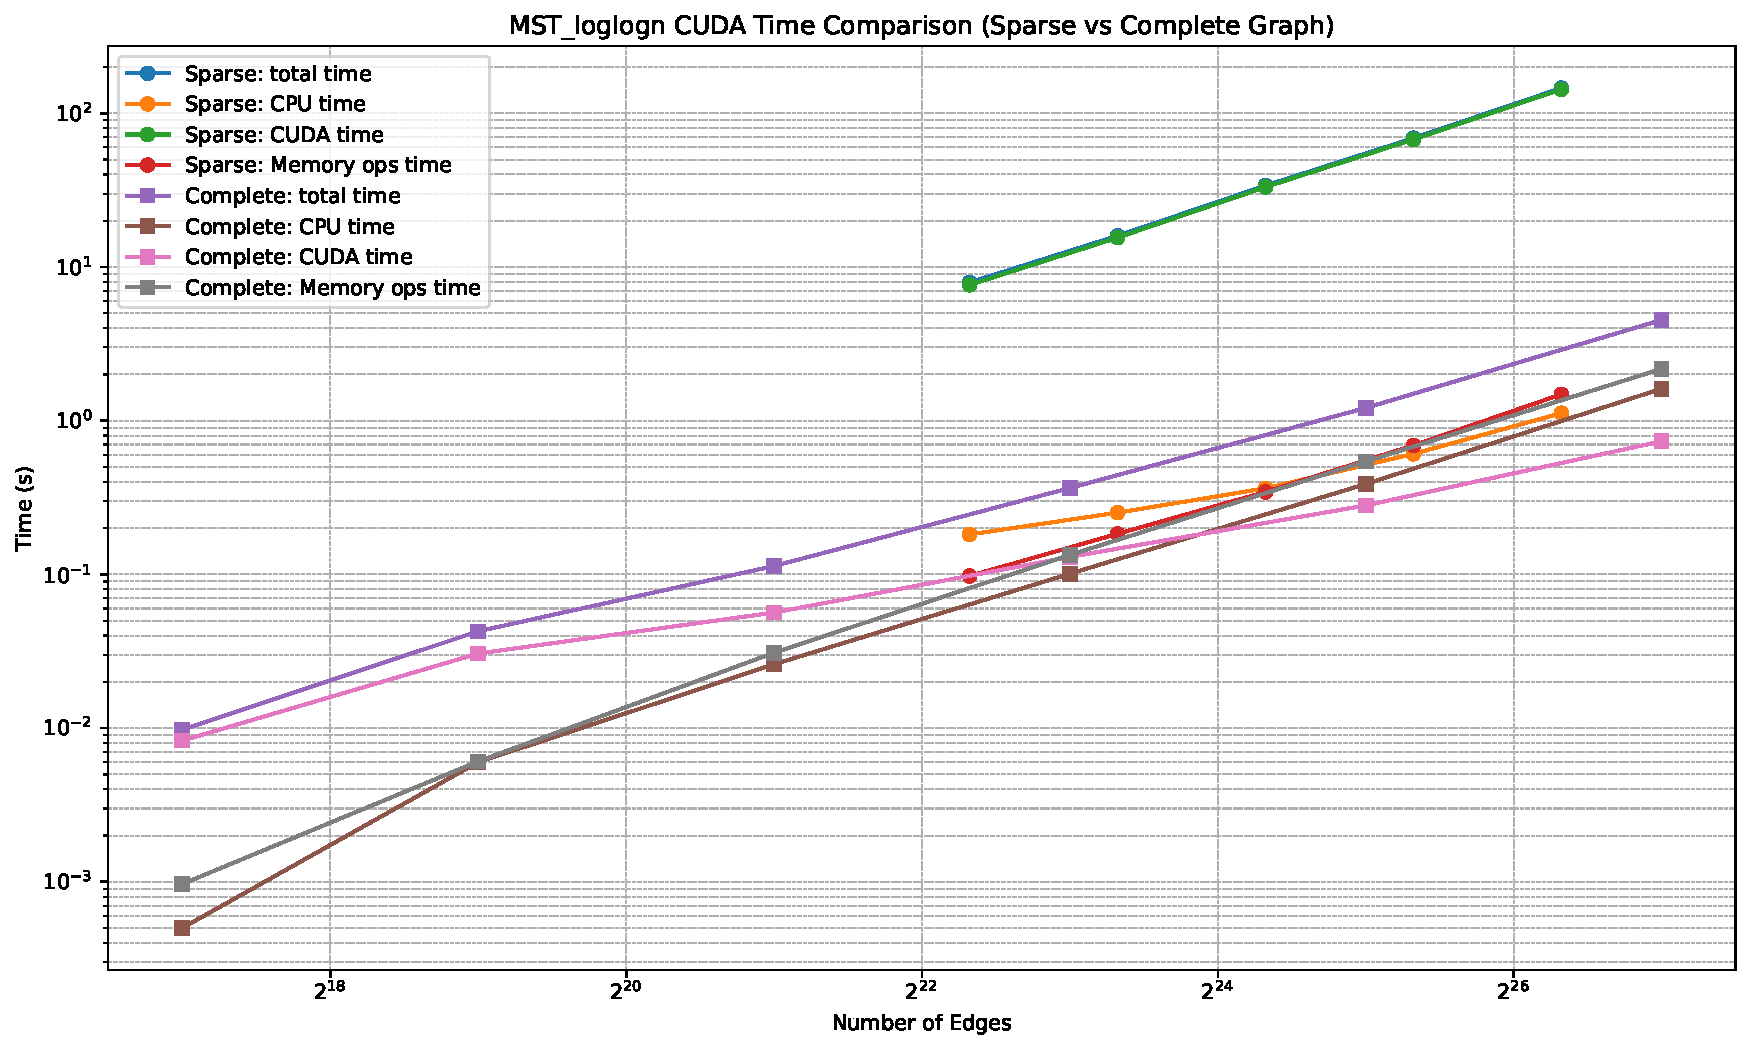
\includegraphics[height=70mm]{cuda_composition_comparison.pdf}
	\caption{\mstalgo{} CUDA time comparison with complete and sparse graph}
	\label{fig:cuda_composition_comparison.pdf}
\end{figure}

In the kernel \texttt{min\_from\_cluster\_kernel}, there a nested loop

% More clusters (inner loop. more time in from edges the kernels)
% We don't know where is the edge to v for example in the buffer. We have to loop through all the edges to find the edge to v. 
% Number of clusters: 4093
% Number of clusters: 162
% Number of clusters: 1

% Number of clusters: 20512
% Number of clusters: 725
% Number of clusters: 1

% N^2 loop in the to cluster so faster growth.
%  it didn't take more rounds in the end. 2 rounds

\subsection{Comparison with Prim's on single threaded CPU}
\begin{figure}[h]
	\centering
		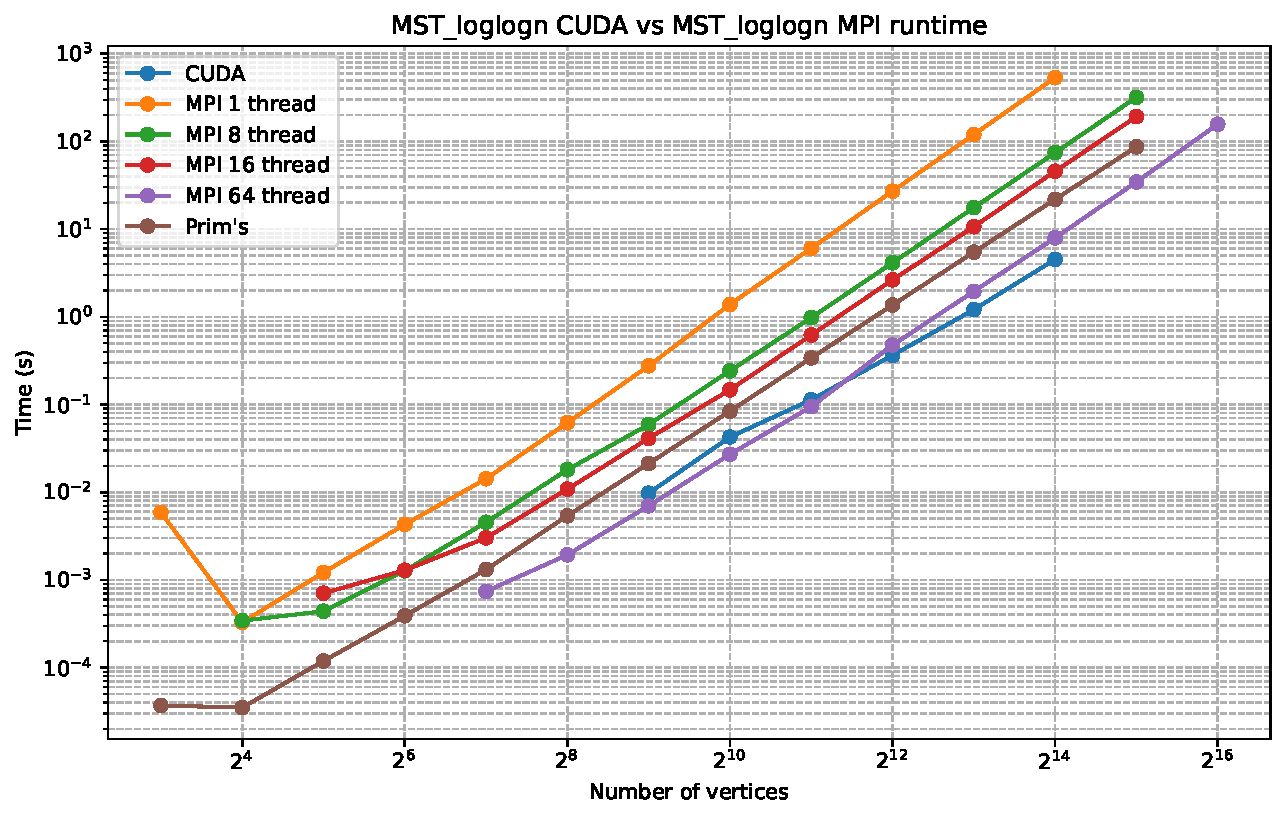
\includegraphics[height=70mm]{CUDA_vs_MPI.pdf}
	\caption{\mstalgo{} CUDA time comparison with MPI and Prim's algorithm}
	\label{fig:CUDA_vs_MPI.pdf}
\end{figure}

Compared with the vanilla Prim's algorithm, the CUDA implementation is significantly faster, with a slower grow in time as the graph size grows, according to \cref{fig:CUDA_vs_MPI.pdf}. While the single-threaded MPI implementation is the slowest, it beats the prim's algorithm when the number of threads is larger than $64$. With $64$ threads, the performance is comparable to the CUDA implementation but with steeper slope.
\clearpage
\section{Conclusion}
\label{sec:conclusion}
When simulating the Congested Clique model with MPI on CPU threads, limited thread resources necessitate vertex partitioning. With few vertices per rank, communication time dominates, but as graph size increases, computation time becomes the bottleneck. Comparing \mstalgo with Prim's algorithm, \mstalgo requires more compute and memory but outperforms Prim's in wall clock time with more work nodes and handles larger graphs. The bottleneck for larger graphs is MPI message memory. The number of rounds is $O(\log{\log{n}})$, as predicted. Python is significantly slower than C++ due to larger memory usage for MPI messages and slower computation, making it more memory-bound.

The high parallelism of the GPU makes it good at parallelize the vertex workload very well. The assignment of the vertex to the thread is very natural. However, when comes to clique graphs, how to fit graphs into vram is a challenge. The high parallelism can be underutilized if the graph is too large to fit into the vram. Sparser graphs show better affinity to the memory-compute trade-off of the GPU.

However, Congested Clique algorithms are often not optimized to run on GPUs. The computation paradigm shows characteristics of CPU computation. Branching in the algorithms brings divergence among the threads on the same SIMT unit, potentially causing the performance to degenerate. Moreover, it is not intuitive to implement the communication between threads. Is it often required that one thread is globally accessible by another even if they are not in the same block. With this constraint, is it not intuitive how to utilize the shared memory of the block. We have to read and write to the vram, which is designed to be slower than the shared memory. We are also missing some matrix operations that are common in the GPU programming, such as MFMA, MMA operations, and their underlying hardware support such as tensor cores.

TODO insert more CUDA conclusion here.

\clearpage
\section{Future work}
\label{sec:future}
How different datatypes affect the performance. We tried double precision, but how about single precision? Hardware typically have different support on different datatypes. E.g. on GPU, single / half precision has better support than double precision.

Can we optimize the algorithm to comply with the GPU architecture better? E.g. how to utilize the shared memory better? How to reduce the divergence among the threads? How to utilize the tensor cores?

\clearpage
%% Bibliography/ list of references
%%
\thesisbibliography

\begin{thebibliography}{99}

	\bibitem{MSTLogLogn} 
	Zvi Lotker, Boaz Patt-Shamir, Elan Pavlov, and David Peleg, "MST Construction in $O(\log{\log{n}})$ Communication Rounds," 
	\textit{SIAM Journal on Computing}, vol. 35, no. 1, pp. 120–131, 2005. 
	\url{https://doi.org/10.1137/S0097539704441848}
	
	\bibitem{powerCongestClique} 
	M. Ghaffari, F. Kuhn, and C. Lenzen, "On the power of the congested clique model," 
	\textit{Proceedings of the 2013 ACM Symposium on Principles of Distributed Computing (PODC '13)}, pp. 367–376, 2013. 
	\url{https://www.researchgate.net/publication/266659337_On_the_power_of_the_congested_clique_model}
	
	\bibitem{Puhti} 
	"Puhti supercomputer," CSC - IT Center for Science. 
	\url{https://research.csc.fi/-/puhti}
	
	\bibitem{PuhtiService} 
	"Puhti Service Description," CSC - IT Center for Science, Jun. 2021. 
	\url{https://research.csc.fi/documents/48467/640068/Puhti-servicedescription-0621.pdf/e6fd32ae-92ea-2d42-0b6c-9f73c1a4c418?t=1628595451763}
	
	\bibitem{PuhtiDoc} 
	"Puhti Computing Systems," CSC - IT Center for Science. 
	\url{https://docs.csc.fi/computing/systems-puhti/}
	
	\bibitem{Slurm} 
	"Slurm Overview," SchedMD. 
	\url{https://slurm.schedmd.com/overview.html}
	
	\bibitem{MPI} 
	"MPI Forum." 
	\url{https://www.mpi-forum.org/}
	
	\bibitem{OpenMPI} 
	"Open MPI." 
	\url{https://www.open-mpi.org/}
	
	\bibitem{HPCScaling} 
	"HPC Scaling," HPC Wiki. 
	\url{://hpc-wiki.info/hpc/Scaling}
	
	\bibitem{V100Architecture} 
	"NVIDIA Volta Architecture," NVIDIA Corporation, White Paper, 2017. 
	\url{https://images.nvidia.com/content/volta-architecture/pdf/volta-architecture-whitepaper.pdf}
	
	\bibitem{CUDA} 
	"CUDA C++ Programming Guide," NVIDIA Corporation. 
	\url{https://docs.nvidia.com/cuda/cuda-c-programming-guide/index.html}
	
	\bibitem{Prufer} 
	H. Prüfer, "Neuer Beweis eines Satzes über Permutationen," 
	\textit{Archiv der Mathematischen Physik}, vol. 27, pp. 742–744, 1918.
	
	\bibitem{IBMsupercomputing} 
	"Supercomputing," IBM. 
	\url{https://www.ibm.com/topics/supercomputing}
	
	\bibitem{MSTConstant} 
	K. Nowicki, "A deterministic algorithm for the MST problem in constant rounds of congested clique," 
	\textit{arXiv.org}, Dec. 9, 2019. 
	\url{https://arxiv.org/abs/1912.04239}
	
	\bibitem{MSTLogStar} 
	M. Ghaffari and M. Parter, "MST in Log-Star rounds of congested clique," 
	\textit{ACM}, 2016. 
	\url{https://doi.org/10.1145/2933057.2933103}
	
	\bibitem{FatTrees} 
	"Fat-Tree Design," Cluster Design. 
	\url{https://clusterdesign.org/fat-trees/}
	
	\bibitem{OpenMPIRepoGather} 
	"Open MPI gather operation," Open MPI. 
	\url{https://github.com/open-mpi/ompi/blob/main/ompi/mpi/c/gather.c}
	
	\bibitem{MPICollective} 
	"MPI tutorial: collective communication," Open MPI. 
	\url{https://mpitutorial.com/tutorials/mpi-broadcast-and-collective-communication/}
	
	\bibitem{PythonInt} 
	"CPython API documentation: Integer Objects," The Python Software Foundation. 
	\url{https://docs.python.org/3/c-api/long.html}
	
	\bibitem{PythonFloat} 
	"CPython API documentation: Floating-Point Objects," The Python Software Foundation. 
	\url{https://docs.python.org/3/c-api/float.html}

	\bibitem{Simtarch} "CUDA C programming SMIT architecture" NVIDIA Corporation, 2025. [Online]. Available: \url{https://docs.nvidia.com/cuda/cuda-c-programming-guide/#simt-architecture}

	\bibitem{Prufer1918} Heinz Prüfer, "Neuer Beweis eines Satzes über Permutationen,"  \textit{Archiv der Mathematik und Physik}, vol. 27, pp. 742–744, 1918.

	\bibitem{Nvprof} "Profiler User’s Guide" NVIDIA Corporation, 2025. [Online]. Available: \url{	https://docs.nvidia.com/cuda/profiler-users-guide/}

	\bibitem{MSTO1Rounds} 
	Tomasz Jurdzinski and Krzysztof Nowicki, "MST in O(1) Rounds of the Congested Clique," 
	\textit{arXiv.org}, Jul. 26, 2017. 
	\url{https://arxiv.org/abs/1707.08484}
\end{thebibliography}


\end{document}
